% !TeX root = main.tex
\chapter{Algoritmi di ordinamento} 
Il problema dell'ordinamento è un problema molto comune e spesso è il passo base per risolvere problemi più complessi.\smallskip\\
\textit{Esempio.}\\
Vogliamo mettere in ordine alfabetico una lista di studenti prenotati ad un esame, perciò é necessario avere:
\begin{itemize}[label=--]
    \item un insieme di elementi
    \item un criterio in base a cui vogliamo ordinare
\end{itemize}

\noindent Definiamo il problema dell'ordinamento come segue:
\newline\textbf{input} $\rightarrow$ una sequenza di $n$ elementi $< a, b, c,..., d>$
\newline \textbf{output} $\rightarrow$ una permutazione $< a', b', c',..., d' >$ della sequenza di input tale che $a' \leq b' \leq \dots \le d'$

\begin{figure}[H]
    \centering
    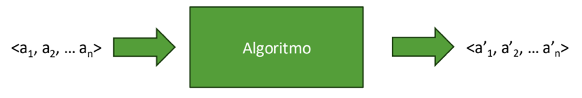
\includegraphics[width=0.5\linewidth]{../images/image3.png}
    \label{Algoritmo}
\end{figure}

\noindent \colorbox{SALZO}{\parbox{\dimexpr\linewidth-2\fboxsep}{\begin{definition}
   (Istanza) L'istanza di un problema è formata dall'input richiesto per calcolare una soluzione del problema.
\end{definition}}}\medskip\\

\noindent \colorbox{SALZO}{\parbox{\dimexpr\linewidth-2\fboxsep}{\begin{definition}
  (Algoritmo corretto) Algoritmo si dice corretto relativamente ad un problema computazionale se, per ogni istanza fornita in input esso:
\begin{enumerate}
    \item Termina
    \item Restituisce una soluzione corretta per l'istanza considerata 
\end{enumerate}
\end{definition}}}\medskip\\

\subsubsection{Algoritmi In-Place}
Alcuni algoritmi di ordinamento possono ordinare una lista senza crearne una nuova. Questi sono conosciuti come algoritmi di orinamento in loco (o in place) e richiedono uno spazio di memoria extra costante O(1). InsertionSort e QuickSort sono \textsc{in-place}, in quanto gli elementi vengono spostati internamente all'array e non allocano memoria aggiuntiva. MergeSort non è \textsc{in place}, richiede memoria aggiuntiva per i diversi frammenti generati.\smallskip\\
\colorbox{SALZO}{\parbox{\dimexpr\linewidth-2\fboxsep}{\begin{definition}
    (Definizione 1) Un algoritmo si definisce \textsc{in place} quando è in grado di restituire l'output utilizzando soltanto un piccolo e costante spazio di memoria extra, i dati in ingresso sono solitamente sovrascritti.
\end{definition}}}\smallskip\\ 
\colorbox{SALZO}{\parbox{\dimexpr\linewidth-2\fboxsep}{\begin{definition}
    (Definizione 2) Un algoritmo si dice \textsc{in place} se al crescere dell'input non crescono le variabili di appoggio.
\end{definition}}}

\section{Insertion Sort}
Insertion Sort è un algoritmo di ordinamento molto semplice che ordina l'insieme di input come farebbe un umano per un mazzo di carte

\begin{enumerate}
    \item inizialmente tutte le carte sono nel mazzo disordinato (input).
    \item prendiamo la prima carta e la teniamo con la mano sinistra.
    \item prendiamo la seconda carta, la confrontiamo con la prima e la posizioniamo alla sua destra o alla sua sinistra in base alla loro relazione d'ordine.
    \item prendiamo la terza carta, la confrontiamo con quelle che abbiamo in mano e la sistemiamo nel posto giusto .
    \item ripetiamo l'operazione di prendere una nuova carta e sistemarla nel posto giusto finché il mazzo non è finito.
\end{enumerate}
\noindent \subsection{Pesudocodice InsertionSort}:
\begin{verbatim}
    INSERTION-SORT(A,n)
    for i = 2 to n
        key = A[i]
        // inserisce A[i] nella sequenza ordinata A[1:i-1]
        j = i - 1
        while j > 0 and A[i] > key
            A[j + 1] = A[j]
            j = j - 1
        A[j + 1] = key
\end{verbatim}
\noindent L'indice i identifica la carta corrente che viene inserita nella mano sinistra. All'inizio di ogni iterazione del ciclo for, il cui indice è $i$, il sotto-array formato dagli elementi $A[1 : i-1]$ costituisce la mano di carte correntemente ordinate, mentre il sotto-array $A[i+1 : n]$ corrisponde alla pila di carte ancora sul tavolo. In effetti, gli elementi $A[1: i-1]$ sono quelli che originariamente occupavano le posizioni da 1 a $i-1$, ma che adesso sono ordinati. Definiamo formalmente queste proprietà soddisfatte da $A[i: i-1]$ in forma di invariante di ciclo.

\begin{figure}[H]
    \centering
    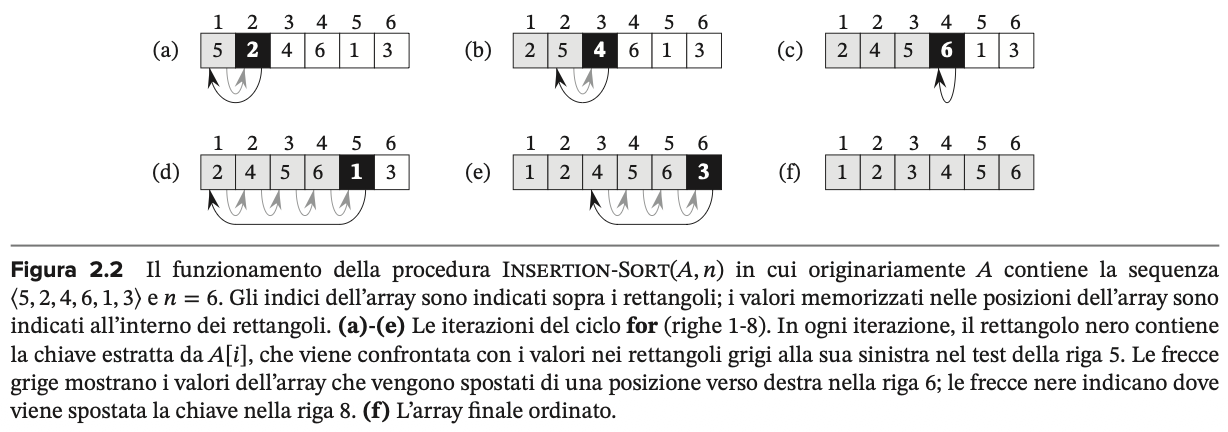
\includegraphics[width=1\linewidth]{../images/Screenshot 2026-03-07 alle 15.31.09.png}

\end{figure}

\subsection{Analisi dell'insertion sort}
Per prima cosa, dobbiamo comprendere che il tempo di esecuzione dipende dall'input, ovviamente ordinare più numeri richiederà più tempo. 
Per analizzare la procedura insertion-sort, la scriviamo qua sotto indicando a fianco di ogni istruzione il costo temporale e il numero di volte per cui viene eseguita. 

\begin{figure}[H]
    \centering
    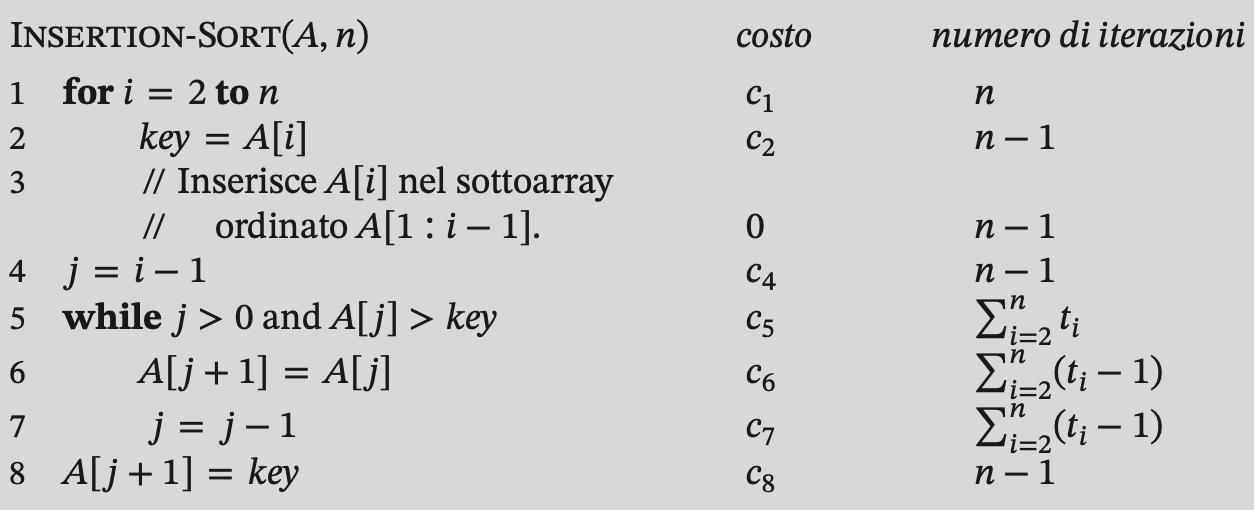
\includegraphics[width=0.6\linewidth]{../images/Screenshot 2026-03-09 alle 18.03.59.png}
    
\end{figure}

\noindent Il tempo di esecuzione dell'algoritmo è la somma dei tempi di esecuzione per ogni istruzione eseguita; un'istruzione che richiede $c_k$ passi viene eseguita m volte contribuirà con $c_k \cdot m$ al tempo di esecuzione totale. Indicheremo il tempo di esecuzione di un algoritmo su un input di dimensione n con T(n). Per calcolare T(n), il tempo di esecuzione di insertion-sort con un input di n valori, sommiamo i prodotti delle colonne costo e numero di volte ottenendo:\\
$$T(n) = c_1n + c_2(n-1) + C_4(n-1) + c_5 \sum_{i=2}^{n}(t_i-1) + c_8(n-1)$$\\
Per insertion-sort il caso migliore si verifica quando l'array è già ordinato. Il tempo di esecuzione nel caso migliore è\\
$$T(n)=c_1n+c_2(n-1)+c_4(n-1)+c_5(n-1)+c_8(n-1)=(c_1+c_2+c_4+c_5+c_8)n-(c_2+c_4+c_5+c_8)$$\\
\noindent Questo tempo di esecuzione può essere espresso come an+b, dove a e b sono costanti che dipendono dai costi $c_k$ delle istruzioni; quindi la funzione che esprime il tempo di esecuzione è una funzione lineare rispetto a n.\\
Il caso peggiore si verifica quando l'array è ordinato in senso inverso, cioè in ordine decrescente. il tempo di esecuzione della procedura insertion-sort nel caso peggiore è
$$T(n)=c_1n+c_2(n-1)+c_4(n-1)+c_5(\frac{n(n+1)}{2}-1)+c_6(\frac{n(n-1)}{2})+c_7(\frac{n(n-1)}{2})+c_8(n-1)=$$\\$$=(\frac{c_5}{2}+\frac{c_6}{2}+\frac{c_7}{2})n^2+(c_1+c_2+c_4+\frac{c_5}{2}-\frac{c_6}{2}-\frac{c_7}{2}+c_8)n-(c_2+c_4+c_5+c_8)$$\\
Questo tempo di esecuzione può essere espresso come $an^2+bn+c$, dove a, b e c sono costanti che dipendono dai costi delle istruzioni $c_k$; quindi è una funzione quadratica rispetto a n.\\
Noi ci concentreremo solo sulla ricerca del tempo di esecuzione nel caso peggiore per tre ragioni:
\begin{enumerate}
    \item il tempo di esecuzione nel caso peggiore di un algoritmo fornisce un limite superiore al tempo di esecuzione su un qualsiasi input. 
    \item per alcuni algoritmi, il caso peggiore si verifica molto spesso. 
    \item il "caso medio" spesso ha un costo simile a quello peggiore. 
\end{enumerate}
\noindent La velocità con cui cresce il tempo di esecuzione, ossia il suo tasso di crescita, è quello che effettivamente ci interessa. Di conseguenza consideriamo soltanto il termine principale di una formula, in quanto i termini di ordine inferiore sono relativamente poco significativi per grandi valori n. Ignoriamo anche il coefficiente costante del termine principale, in quanto i fattori costanti sono meno significativi del tasso di crescita nel determinare l'efficienza computazionale per grandi input. per il tempo di esecuzione del caso peggiore dell'insertion-sort, se ignoriamo i termini di ordine inferiore e il coefficiente del termine principale, resta solo il fattore $n^2$ che fa parte del termine principale.\\
Utilizzeremo la notazione $\Theta(costo)$ per evidenziare l'ordine di crescita del tempo di esecuzione. L'insertion sort ha un tempo di esecuzione nel caso peggiore pari a $\Theta(n^2)$.\\
Un algoritmo è considerato più efficiente di un altro se il suo tempo di esecuzione nel caso peggiore ha un tasso di crescita minore rispetto all'altro.

\subsection{Costi InsertionSort}
Analizzando lo pseudocodice, si può notare che i cicli risultano essere le operazioni più frequenti. Dunque il ciclo for viene eseguito $n-1$ volte, mentre il ciclo while, $j$ volte, tuttavia osservando che il valore $j$ viene inizializzatofuori dal while a $i-1$, si capisce che l'ultimo valore sarà prorpio $j = (n-1)-1 = n-2$. Da ciò è possibile intuire che il  costo dell'algoritmo sarà $(n-1) \cdot (n-2)$, ovvero il costo asintotico sarà pari a $O(n^2)$.\\

\noindent Dobbiamo fornire una \textbf{prova di correttezza}, ossia una dimostrazione formale che non considera un input specifico ma ragiona sull'algoritmo, sulle proprietà dell'input e su come viene prodotto l'output

\begin{itemize}[label=--]
    \item esistono molte tecniche per dimostrare la correttezza di un algoritmo rispetto ad un problema, come la tecnica degli invarianti di ciclo
\end{itemize}

\noindent \section{Invariante di ciclo}
È una tecnica per dimostrare che un particolare algoritmo risolve correttamente un dato problema. Ci sono tre cose che devono essere dimostrate:

\begin{enumerate}
    \item Inizializzazione $\rightarrow$ esiste una proprietà che vale prima dell'iterazione del ciclo
    \item Mantenimento $\rightarrow$ se la proprietà vale prima del ciclo, allora rimane vera anche prima dell'iterazione successiva
    \item Conclusione $\rightarrow$ il ciclo termina e la proprietà che preserviamo dimostra che il risultato è corretto
\end{enumerate}

\noindent \colorbox{SALZO}{\parbox{\dimexpr\linewidth-2\fboxsep}{\begin{definition}
    (Invarianza di ciclo) Una dimostrazione di invarianza di ciclo è una forma di dimostrazione per induzione matematica, dove per provare che una proprietà è valida. si prova un caso base e un passo induttivo.\\
    Nel nostro caso, dimostrare che l'invariante è vera prima della prima iterazione corrisponde al caso base, mentre dimostrare che l'invariante resta vera da un'iterazione all'altra corrisponde al passo induttivo.
\end{definition}}}\\

\subsubsection{Inizializzazione}
Iniziamo dimostrando che l'invariante di ciclo è vera prima della prima iterazione del ciclo, cioè quando $i=2$. Il sottoarray $A[i : i-1]$ è formato dal solo elemento $A[1]$, che infatti è l'elemento originale in $A[1]$. Inoltre, questo sottoarray è ordinato, il che dimostra che l'invariante di ciclo vale prima della prima iterazione del ciclo.

\subsubsection{Mantenimento}
Passiamo alla seconda prorpietà: dimostrare che ogni iterazione conserva l'invariante di ciclo. Informalmente, il corpo del ciclo for esterno opera spostando $A[i-1]$, $A[i-2]$, $A[i-3]$ e cosi cia di una posizone verso destra, finché non troverà la posizione appropriata per $A[i]$, in cui inserirà il valore di $A[i]$. Il sottoarray $A[1 : i]$ quindi è ordinato ed è formato dagli stessi elementi che originariamente erano in $A[1 : i]$. Dunque, l'incremento di $i$ per la successiva iterazione del ciclo for preserva l'invariante di ciclo.

\subsubsection{Conclusione}
Infine, esaminiamo che cosa accade quando il ciclo termina. La variabile del ciclo $i$ viene inizializzata a 2 e aumenta di 1 a ogni iterazione. Non appena il valore di $i$ eccede $n$ nella linea 1, il ciclo termina. Detto in altro modo: il ciclo termina non appena $i$ assume il valore $n+1$. Sostituendo $n+1$ a $i$ nella formulazione dell'invariante del ciclo, si trova che il sotto-array $A[1 : n]$ consiste degli elementi originariamente presenti in $A[1 : n]$, ma ordinati. Pertanto l'algoritmo è corretto.

\section{Divide et impera}
Dato un problema possono esistere diversi algoritmi in grado di risolverlo. Generalmente gli algoritmi ricorsivi adottano un approccio del tipo divide et impera.

\begin{itemize}
    \item Divide
        \begin{enumerate}
            \item il problema viene diviso in un certo numero di sottoproblemi
            \item tali sottoproblemi sono istanze più piccole del problema originale
        \end{enumerate}
    \item Impera
        \begin{enumerate}
            \item i sottoproblemi vengono risolti in modo ricorsivo
            \item si continua a dividere fino ad arrivare ad una istanza sufficientemente piccola da essere risolta direttamente
        \end{enumerate}
    \item Combina
    \begin{enumerate}
            \item Le soluzioni dei sottoproblemi vengono combinate per formare la soluzione del problema originale
        \end{enumerate}
\end{itemize}

\section{Merge sort}
L'algoritmo merge sort segue da vicino la strategia divide et impera. A ogni passo, ordina un sotto-array $A[r : p]$, partendo dall'intero array $A[1: n]$ e operando ricorsivamente su sotto-array sempre più piccoli.
\begin{itemize}
    \item Divide
    \begin{enumerate}
        \item Se la lista contiene più di un elemento spezzala in due sotto-liste grandi la metà. Per fare ciò clacola il centro q del sottoarray A[p : r] e divide A[p : r] nei sottoarray A[p : q] e A[q+1 : r].
    \end{enumerate}
    \item Impera
    \begin{enumerate}
        \item Continua a dividere finché la lista non ha dimensione 1. Quindi ordina ciascuno dei sottoarray in modo ricorsivo utilizzando l'algoritmo merge sort
    \end{enumerate}
    \item Combina
    \begin{enumerate}
        \item Fonde due sotto-liste ordinandole
    \end{enumerate}
\end{itemize}

\vspace{1cm}

\noindent \subsection{Pseudocodice MergeSort}
\begin{verbatim}
    MERGE-SORT(A,p,r)
    if p >= r               //zero o un solo elemento?
        return
    q=|(p+r)/2|             //punto medio di A[p : r]
    MERGE-SORT(A,p,q)       //ordina ricorsivamente A[p : q]
    MERGE-SORT(A,q+1,r)     //ordina ricorsivamente A[q+1 : r]
    //fonde A[p : q] con A[q+1 : r] in A[p : r]
    MERGE(A,p,q,r)
\end{verbatim}

\noindent pseudocodice merge (metodo, combina, che fonde due sotto-liste ordinate):
\begin{verbatim}
    MERGE(A,p,q,r)
    n_l = q - p + 1         //lunghezza di A[p : q]
    n_r = r - q             //lunghezza di A[q+1 : r]
    crea due nuovi array L[0 : n_l -1] e R[0 : n_r -1]
    for i =0 to n_l -1      //copia A[p : q] in L[0 : n_l -1]
        L[i] = A[p + i]
    for j = 0 to n_r -1     //copia di A[q+1 : r] in R[0 : n_r - 1]
        R[j] = A[q + j + 1]
    i = 0                   //i è l'indice del più piccolo elemento che resta in L
    j = 1                   //i è l'indice del più piccolo elemento che resta in R
    k = p                   //k è la posizione di A in cui fare il prossimo inserimento
    //finchè L e R contengono un elemento non ancora fuso,
    //copia il più piccolo elemento non fuso in A[p : r]
    while i < n_l
       if L[i] <= R[j]
             A[k] = L[i]
             i = i + 1
        else A[k] = R[j]
            j = j + 1
        k = k + 1
    //avendo esaurito completamente uno tra L e R,
    //copia il resto dell'altro nella porzione finale di A[p : r]
    while i < n_l
        A[k] = L[i]
        i = i + 1
        k = k + 1
    while j < n_r
        A[k] = R[j]
        j = j + 1
        k = k + 1
\end{verbatim}
\noindent esempio:\\
\begin{figure}[H]
    \centering
    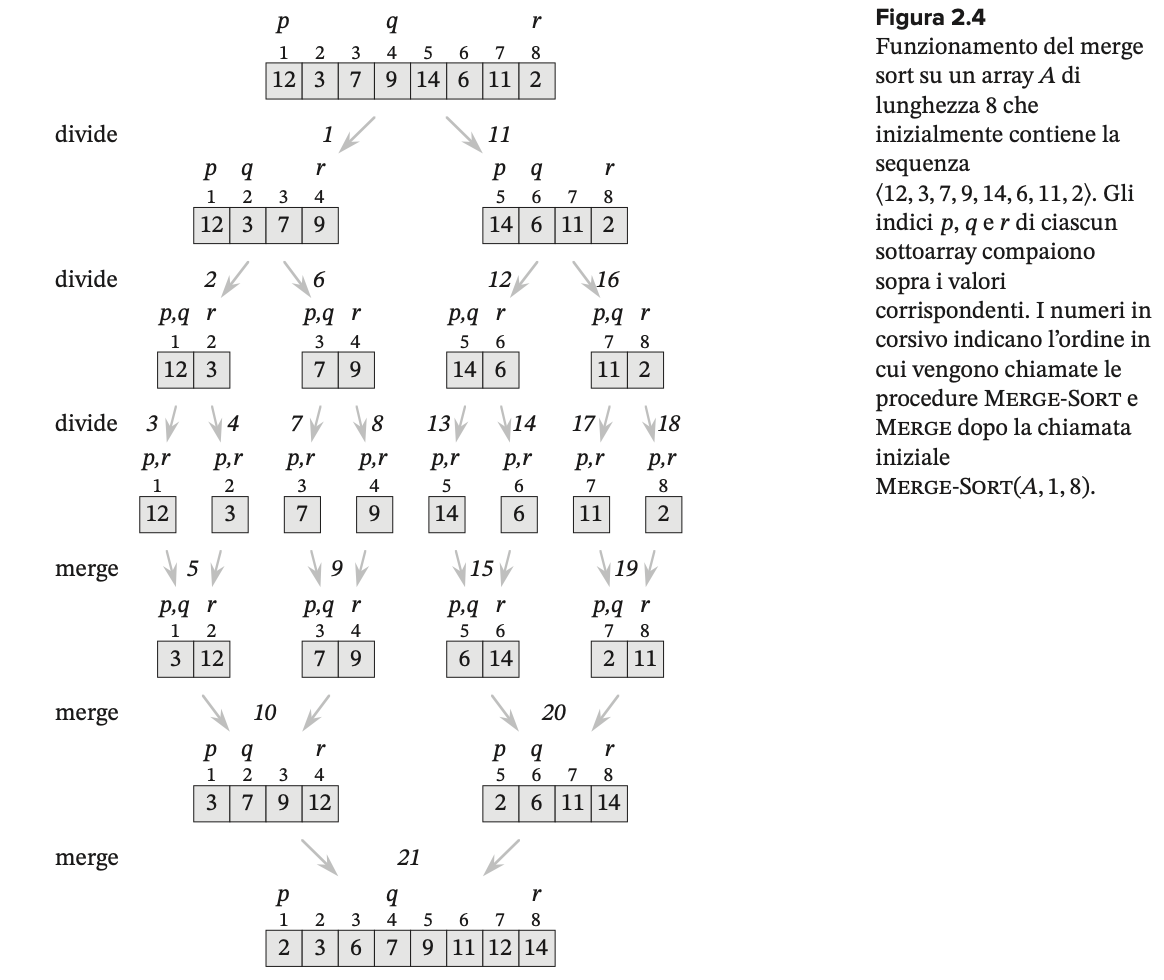
\includegraphics[width=0.8\linewidth]{../images/Screenshot 2026-03-10 alle 17.47.34.png}
\end{figure}

\subsection{Analisi del MergeSort}
Il MergeSort è un algoritmo efficiente la cui complessità temporale per l’ordinamento di un
intero array di dimensione n è solamente $O(n \log(n))$.\\
L'algoritmo è conforme al paradigma Divide et Impera che viene sviluppato come segue:
\begin{enumerate}
    \item \textbf{Divide}: divide la sequenza degli $n$ elementi da ordinare in due sotto-sequenze di $n/2$ elementi ciascuna.
    \item \textbf{Impera}: ordina le due sotto-sequenze in modo ricorsivo.
    \item \textbf{Combina}: fonde le due sotto-sequenze ordinate per generare la sequenza ordinata finale.
\end{enumerate}
\subsection{Equazione di ricorrenza}
$$
\begin{cases}
    T(n)=2 \cdot T(\frac{n}{2})+O(n) \qquad \text{   passo ricorsivo}\\
    T(1)=1 \qquad \qquad \qquad \qquad \quad \text{passo base}
\end{cases}
$$

\begin{figure}[H]
    \centering
    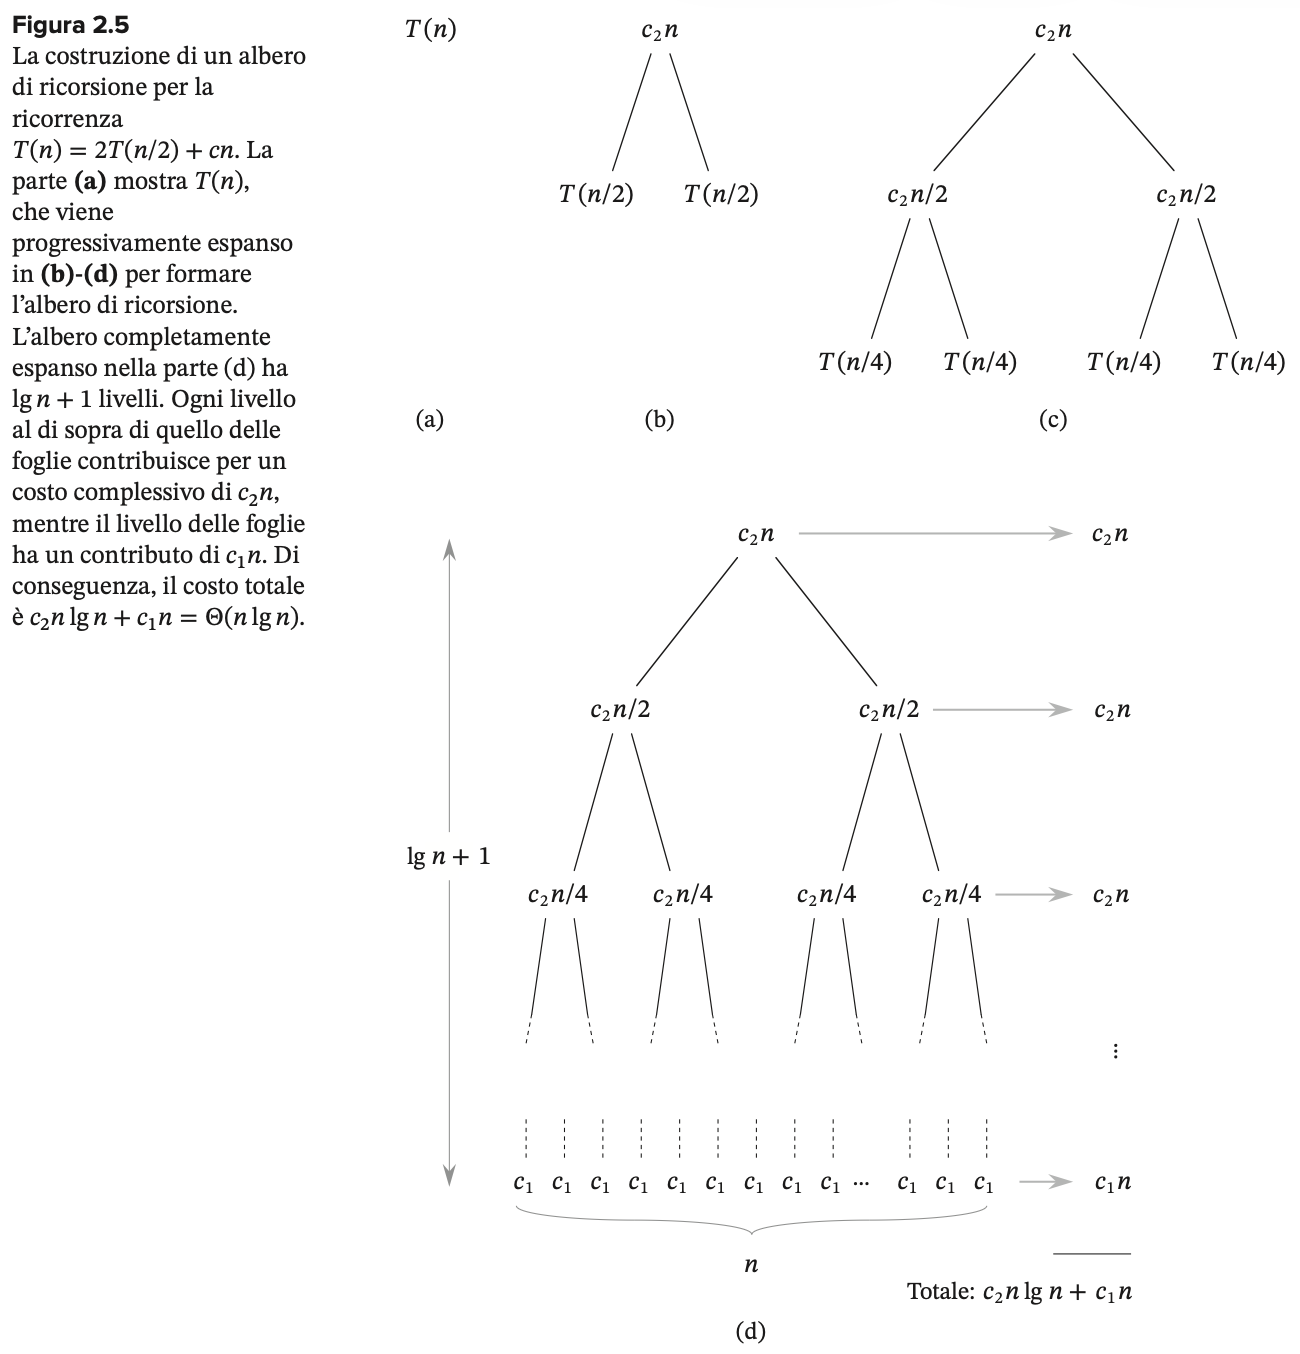
\includegraphics[width=0.8\linewidth]{../images/Screenshot 2026-03-11 alle 08.20.07.png}
\end{figure}

\section{Quick sort}
Il quicksort è un algoritmo di ordinamento il cui tempo di esecuzione nel caso peggiore è $\Theta(n^2)$ su un array di input di n numeri.\\
Questi sono i tre passi del processo divide et impera per ordinare un generico sottoarray $A[p : r]$:
\begin{itemize}
    \item \textbf{Divide}
    \begin{enumerate}
        \item Fissiamo un pivot $q$
        \item Riorganizziamo l'input in due sotto liste, $A[p : q-1]$ (sezione bassa) e $A[q+1 : r]$ (sezione alta)
        \item Nella riorganizzazione dobbiamo garantire che ogni elemento della sezione bassa è $\le$ di ogni elemento della sezione alta
    \end{enumerate}
    \item \textbf{Impera}
    \begin{enumerate}
        \item Ordiniamo le due sotto-liste in modo ricorsivo
    \end{enumerate}
    \item \textbf{Combina}
    \begin{enumerate}
        \item Poiché le due sotto liste sono già ordinate. Tutti gli elementi di $A[p : q-1]$ sono in ordine e $\le$ al pivot $A[q]$, e tutti quelli di $A[q+1 : r]$ sono in ordine e $\ge$ al pivot $A[q]$. Ma allora l'intera lista $A[p : r]$ non può che essere ordinata.
    \end{enumerate}
\end{itemize}

\begin{figure}[H]
    \centering
    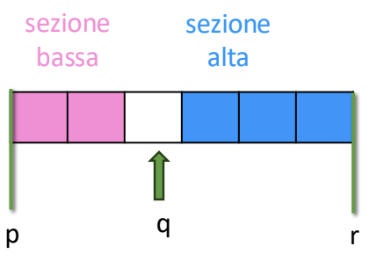
\includegraphics[width=0.25\linewidth]{../images/Screenshot 2026-03-06 alle 10.18.29.png}
    \label{Quick Sort 1}
\end{figure}

\noindent \subsection{Pseudocodice QuickSort}
\begin{verbatim}
QUICKSORT(A,p,r)
1   if p < r
2       //Partiziona il sottoarray intorno al pivot, che finisce in A[q]
3       q = PARTIZIONA(A,p,r)   //calcolo l'indice dell'elemento pivot con partiziona(A, p, r)
4       QUICKSORT(A,p,q-1)      //ordina ricorsivamente la sezione bassa
5       QUICKSORT(A,q+1,r)      //ordina ricorsivamente la sezione alta
\end{verbatim}

\noindent Pseduocodice \texttt{PARTIZIONA}:
\begin{verbatim}
PARTIZIONA(A,p,r)
1   x = A[r]                    //il pivot
2   i = p - 1                   //l'indice più alto nella sezione bassa
3   for j = p to r - 1          //tratta ogni elemento che non è il pivot
4       if A[j] <= x            //questo elemento appartiene alla sezione bassa?
5           i = i + 1           //indice di nuova posizione della sezione bassa
6           scambia A[i] con A[j]   //inserisce questo elemento nella nuova posizione
7   scambia A[i+1] con A[r]     //il pivot si torva a destra della sezione bassa
8   return i + 1                //il nuovo indice del pivot
\end{verbatim}

\noindent \textit{Esempio.} Ordinare il seguente array:

\begin{figure}[H]
    \centering
    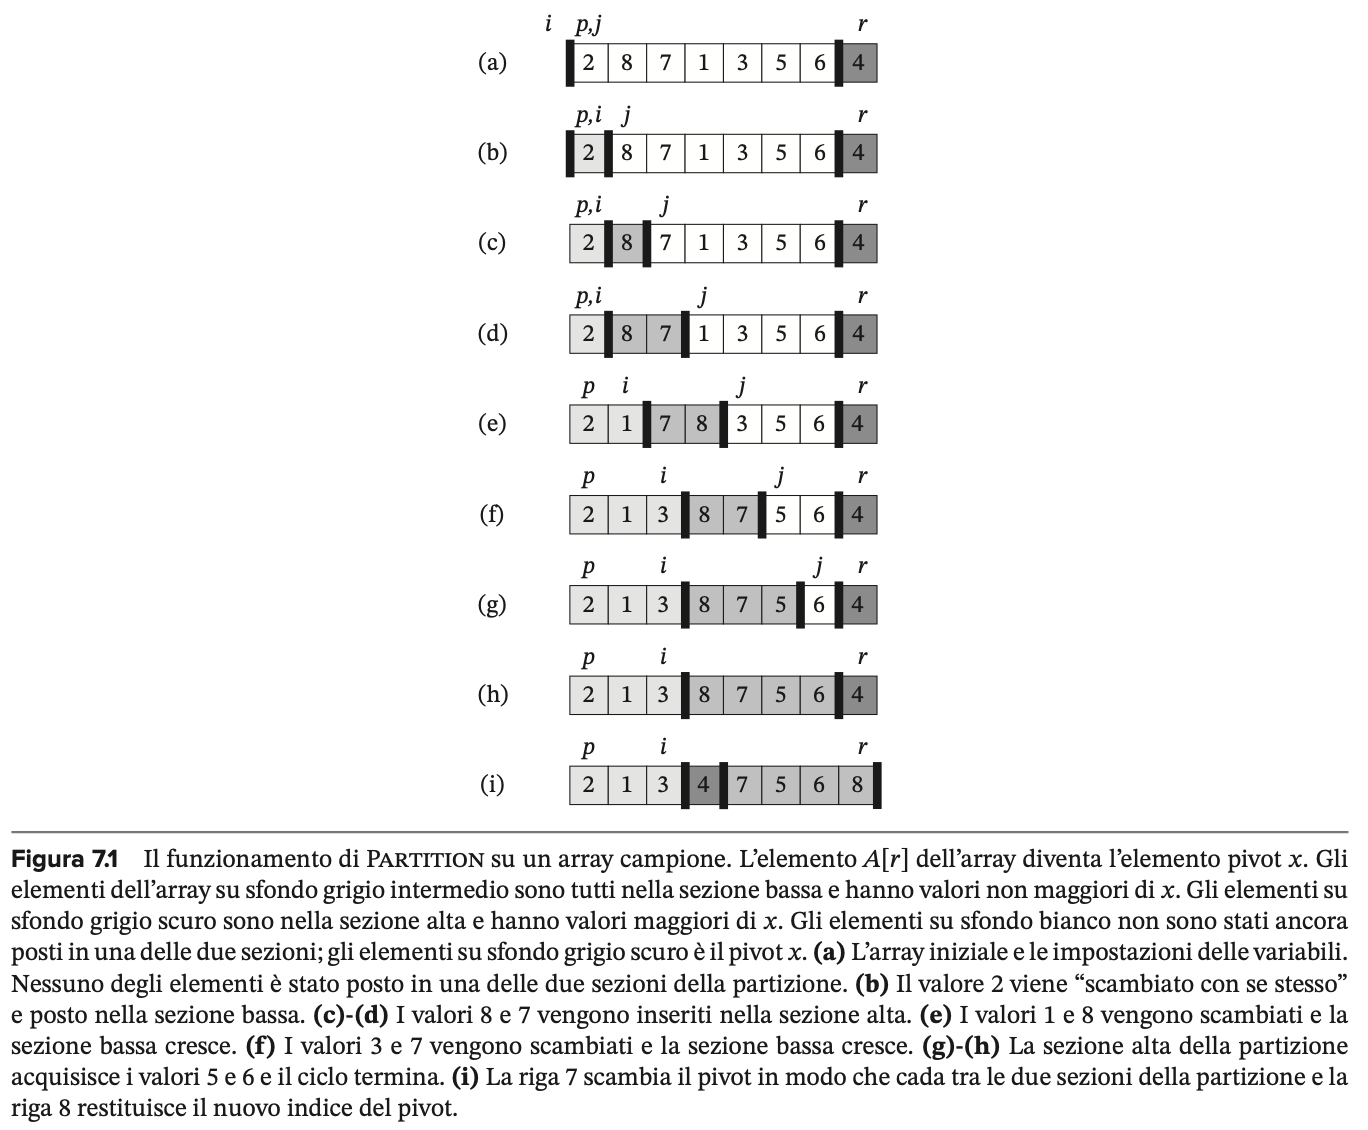
\includegraphics[width=0.70\linewidth]{../images/Screenshot 2026-03-12 alle 22.38.44.png}
\end{figure}
\noindent All'inizio di ogni iterazione del ciclo for, per ogni indice $k$ dell'array valgono le seguenti condizioni:
\begin{enumerate}
    \item se $p \le k\le i$ allora $A[k] \le x$
    \item se $i+1 \le k \le j-1$ allora $A[k]\ge x$
    \item se $k=r$ allora $A[k]=x$
\end{enumerate}
\noindent \subsection{Dimostrazione della correttezza di Quicksort}
Dobbiamo dimostrare che questa invariante di ciclo è vera prima della prima iterazione, che ogni iterazione conserva l'invariante di ciclo, che il ciclo termina e, quando ciò avviene, che la correttezza segue dall'invariante.\\

\noindent \textbf{Passo 1 - Inizializzazione}
\begin{enumerate}
    \item prima della prima iterazione del ciclo si ha $i = p-1$ e $j = p$ 
    \item poiché non ci sono valori fra $p$ e $i$ né fra $i+1$ e $j-1$, le prime due condizioni dell'invariante di ciclo sono banalmente soddisfatte.
    \item l'assegnamento nella riga 1 soddisfa la terza condizione.
\end{enumerate}
\noindent \textbf{Passo 2 - Mantenimento}\\
\textsc{recall}: Dobbiamo dimostrare che ogni iterazione mantiene l'invariante. Supponiamo quindi che sia vera prima della k-esima iterazione e mostriamo che resta vera al temrine\smallskip\\
Nella riga 11 di \texttt{partizione()} controllo se $A[k]$ $\le$ $x$:
    \begin{itemize}
        \item \textsc{caso false}: non succede nulla e si passa alla prossima iterazione.
        \item \textsc{caso true}: viene incrementato l'indice $i$, vengono scambiati $A[i]$ e $A[j]$ e si passa alla prossima iterazione. 
    \end{itemize}


\noindent \textbf{Passo 3 - Conclusione}
\begin{enumerate}
    \item il ciclo termina quando $j=r$
    \item i valori dell'array si trovano ripartiti in tre insiemi: quelli minori o uguali a $x$, quelli maggiori di $x$ e un insieme di un solo elemento che contiene $x$ (il pivot).
    \item viene eseguita la linea 6 del codice \texttt{PARTIZIONA(A,p,r)} e si scambiano $A[i+1]$ e $A[r]$. L'output di \texttt{PARTIZIONA} adesso soddisfa le specifiche del passo divide. Infatti dopo la riga 3 di \texttt{QUICKSORT} $A[q]$ è strettamente minore di ogni elemento in $A[q+1 : r]$. 
\end{enumerate}
\subsection{Prestazioni QuickSort}
il tempo di esecuzione del quicksort dipende da quanto è bilanciata ogni partizione e questo, a sua volta, dipende da quali elementi vengono usati come pivot. Se le due sezioni della partizione hanno all'incirca la stessa dimensione, cioè se è bilanciato, allora l'algoritmo ha un costo $O(n \log n)$. Se il partizionamento è sbilanciato ha un costo $O(n^2)$. Il costo in memoria dell'algoritmo invece è $O(n)$ in quanto non viene allocato nuovo spazio in memoria per i sotto-array, bensì si richiama ricorsivamente sullo stesso. \\
Il caso peggiore del QuickSort è quando l'array da ordinare è già ordinato o è ordinato in ordine inverso, o quando tutti gli elementi sono uguali. \\
Il QuickSort è di per se un algoritmo efficiente, però può essere migliorato abbassando la probabilità di incontrare dei casi sfavorevoli, quindi evitando di incontrare casi di sbilanciamento nei due sotto-array. Per fare questo si utilizza una versione randomizzata del QuickSort, in cui la scelta del pivot avviene in modo pseudo-casuale.
\subsection{Tempo di esecuzione QuickSort}
$$T(n)=
\begin{cases}
    O(1) \qquad \qquad \qquad \qquad \qquad \quad \text{se } n\le 1 \text{ paso base}\\
    T(k)+T(n-k-1)+O(n) \quad \text{se } n > 1 \text{ paso ricorsivo}
\end{cases}$$
\noindent Dove $T(k)$ rappresenta il tempo di esecuzione del QuickSort per il sotto array con $k$ elementi, $T(n-k-1)$ rappresenta il tempo di esecuzione del QuickSort per il sotto array con $n-k-1$ che non includono il pivot scelto, $O(n)$ rappresenta il tempo necessario per effettuare la partizione dell'array in base al pivot, che richiede un tempo lineare proporzionale alla dimensione dell'array. Il passo base dell'equazione di ricorrenza del QuickSort è quando l'array da ordinare contiene zero o un solo elemento, in cui il tempo di esecuzione è costante.

\section{Ricorrenze}
Per analizzare gli algoritmi ricorsivi basati sul metodo divide et impera, abbiamo bisogno di alcuni strumenti matematici. Una \textbf{ricorrenza} è un'equazione che descrive una funzione in termini del suo valore su altri argomenti, in genere più piccoli. Le ricorrenze vengono usate con il meotodo divide et impera perchè ci danno un modo naturale per caratterizzare matematicamente i tempi di esecuzione degli algoritmi ricorsivi.\\
La forma generale di una ricorrenza è un'equazione o una  disequazione che descrive una funzione definita sugli interi o sui reali utilizzando la funzione stessa. Essa contiene due o più casi, a seconda dell'argomento. Se un caso comporta la chiamata ricorsiva della funzione su input diversi, si tratta di un \textbf{caso ricorsivo}. Se un caso non comporta una chiamata ricorsiva, è un \textbf{caso base}.

\subsubsection{Ricorrenze algoritmiche}
 Una ricorrenza T(n) è di natura algoritmica se, per ogni soglia $n_0>0$ sufficientemente grande valgono le seguenti proprietà:
 \begin{enumerate}
     \item per ogni $n<n_0$, si ha $T(n)=\Theta(1)$
     \item per ogni $n \ge n_0$, ogni cammino di ricorsione termina in un caso base entro un numero finito di chiamate ricorsive.
 \end{enumerate}

\section{Impostazione di una ricorrenza}
Tutte le volte che abbiamo un algoritmo ricorsivo, bisogna impostare una \textbf{ricorrenza}.\smallskip\\
\textit{Esempio.}
\begin{verbatim}
    int ricercaBinariaRic(int a[], int primo, int ultimo, int k)
\end{verbatim}
Vogliamo cercare una funzione $T(n)$ che descriva il costo della funzione, il nostro esempio ha questa ricorrenza:
$$\begin{cases}
   \displaystyle T(n)= C+T\left(\frac{n}{2}\right) \qquad n>1 \\
    T(1) = 1 \quad \to \quad \text{caso base} 
\end{cases}$$
Procediamo con uno sviluppo manuale per sostituzione, che chiamiamo per \textbf{Srotolamento}:\\
Dopo aver impostato la ricorrenza, applichiamo la manualmente la ricorsione:
$$n\to \frac{n}{2} :\qquad T\left(\frac{n}{2} \right) = 1 + T\left( \frac{n}{2^2} \right) $$
$$\frac{n}{2}\to \frac{n}{4}:\qquad T\left(\frac{n}{4} \right) = 1+ T\left( \frac{n}{2^3} \right)$$
Quindi riscriviamo l'espressione di $T(n)$ con le sostituzioni che abbiamo fatto sopra:
$$T(n) = 1+\underbrace{1+T\left(\frac{n}{2^2}\right)}_{ \displaystyle T\left(\frac{n}{2}\right)} = 1+1+\underbrace{1+ T\left( \frac{n}{2^3} \right)}_{\displaystyle T\left( \frac{n}{2^2}\right)} = \cdots =  \boxed{ K + T \frac{n}{2^k}}$$\\
Visto che il caso base è $T(1) = 1$, dobbiamo vedere per quale valore di $k$ si ha che $ \frac{n}{2^k} = 1$. Ciò avviene per $k = \log n$, quindi riscriviamo l'espressione di $T(n)$ con questo valore di $k$:
$$T(n)=\log n+1 \quad \in \quad \Theta(\log n)$$
Questo esempio è la dimostrazione di un algoritmo \textbf{In-Place}.\\
Negli algoritmi "in-place" si usa la dimensione dell'input più qualche variabile. Non tutti gli algoritmi possono essere portati "in-place" come ad esempio merge-sort.\bigskip\\

\noindent \textit{Esempio.}

\begin{verbatim}
    MERGE-SORT(A,p,r)
    if p >= r               //zero o un solo elemento?
        return
    q=|(p+r)/2|             //punto medio di A[p : r]
    MERGE-SORT(A,p,q)       //ordina ricorsivamente A[p : q]
    MERGE-SORT(A,q+1,r)     //ordina ricorsivamente A[q+1 : r]
    //fonde A[p : q] con A[q+1 : r] in A[p : r]
    MERGE(A,p,q,r)
\end{verbatim}

\noindent Questo algoritmo ha questo schema di ricorrenza:
$$\begin{cases}
    \displaystyle T(n)=2T\left(\frac{n}{2}\right)+M(n)\\
    T(1) = 1 \quad \to \quad \text{caso base}
\end{cases}$$
Dove $M(n)$ è il costo della chiamata del \texttt{MERGE(A,p,q,r)}, che ancora non conosciamo.\\
Per vedere quanto vale il costo guardiamo il suo pseudocodice:
\begin{verbatim}
    MERGE(A,p,q,r)
    nL = q - p + 1         //lunghezza di A[p : q]
    nR = r - q             //lunghezza di A[q+1 : r]
    //crea due nuovi array 
    L = [0 : nL -1]
    R = [0 : nR -1]
    
    for i = 0 to nL -1      //copia A[p : q] in L[0 : nL -1]
        L[i] = A[p + i]
        
    for j = 0 to nR -1     //copia di A[q+1 : r] in R[0 : nR - 1]
        R[j] = A[q + j + 1]
    i = 0                   //i è l'indice del più piccolo elemento che resta in L
    j = 0                   //i è l'indice del più piccolo elemento che resta in R
    k = p                   //k è la posizione di A in cui fare il prossimo inserimento

    //unisci i due sottoarray in ordine
    while i < nL and j < nR
       if L[i] <= R[j]
             A[k] = L[i]
             i = i + 1
        else A[k] = R[j]
            j = j + 1
        k = k + 1
    
    //avendo esaurito completamente uno tra L e R,
    //copia il resto dell'altro nella porzione finale di A[p : r]
    while i < nL
        A[k] = L[i]
        i = i + 1
        k = k + 1
    while j < nR
        A[k] = R[j]
        j = j + 1
        k = k + 1
\end{verbatim}
\noindent Dallo pseudocodice si evince che il costo di $M(n)$ è $n$, poichè quando vengono copiati gli array in due buffer temporanei, si ha un costo di $\Theta (n)$, poi quando vengono effettuati gli ultimi due cicli per svuotare i buffer, per ogni elemento "spendiamo" una costante, quindi anche in questa fase il costo è di $\Theta(n)$.\smallskip\\
Possiamo quindi riscrivere lo schema di ricorrenza con $M(n) = n$:
$$
\begin{cases}
\displaystyle T(n)=2T\left(\frac{n}{2}\right)+n \\
T(1)=1
\end{cases}
$$
Si procede con lo srotolamento:
$$n\to \frac{n}{2}:\qquad T\left(\frac{n}{2}\right) = 2T\left(\frac{n}{2^2}\right)+\frac{n}{2}$$
$$\frac{n}{2}\to \frac{n}{4}:\qquad T\left(\frac{n}{2^2}\right)=2T\left(\frac{n}{2^3}\right)+\frac{n}{2^3}$$
Quindi $T(n)$ diventa:
$$T(n)= 2T\left( \frac{n}{2} \right) +n = 2\ \underbrace{\left[ 2T\left( \frac{n}{2^2} \right) +\frac{n}{2} \right]}_{\displaystyle T\left( \frac{n}{2} \right)  } + n  = \cdots = \boxed{2^k\  T \left( \frac{n}{2^k} \right)k\ n }$$
Dato il caso base $T(1) = 1$, dobbiamo trovare il valore di $k$ tale che $2^k = 1$, ovvero per $k = \log n$, perciò $T(n)$ diventa:
$$\displaystyle  T(n) = 2^{\displaystyle \log n} \ T(1)+\log n \cdot n = n + n \log n \quad \in \Theta(n \log n )$$
\bigskip\\
\textit{Esempio.}\\
Si ha la seguente ricorrenza:
$$\begin{cases}
    T(n) = T(n-1) +n\\
    T(1) = 1 \quad \to \quad \text{caso base}
\end{cases}$$
Applichiamo lo srotolamento:
$$n\to n-1:\qquad T(n-1) = T(n-2)+n-1$$
$$n-1 \to n-2: \qquad T(n-2) = T(n-3)+n-2$$
Sostituendo a $T(n)$ diventa:
$$T(n) = T(n-3) +(n-2) + (n-1) + n = \cdots =  \boxed{T(n-k)+\sum_{i=0}^{k-1}{(n-i)}}$$
Semplifichiamo la sommatoria:
$$\sum_{i}^{k-1}{(n-i)}=\sum_{i}^{k-1}{n}-\sum_{i}^{k-1}{i}=k \cdot n-\frac{(k-1)(k-2)}{2}$$\\
dove per la seconda sommatoria abbiamo usato il criterio di Gauss.\\
Ora per il caso base $T(1) =1$, troviamo che $n-k = 1$ quando $k = n-1$, sostituendo si ottiene:
$$T(n)=(n-1) \cdot n - \frac{(n-2)(n-3)}{2} = 1+\frac{2n^2-2n-n^2-3n-2n-6}{2} \quad \in \Theta(n^2)$$
\bigskip\\
\textit{Esempio.}\\
Si ha la seguente ricorrenza:
 $$
\begin{cases}
\displaystyle T(n)=T\left(\frac{n}{2}\right)+\frac{n}{2}\\
T(1)=1\quad \to \quad \text{caso base} 
\end{cases}$$
Applichiamo lo srotolamento:
$$n\to \frac{n}{2}:\qquad T\left(\frac{n}{2}\right)=T\left(\frac{n}{2^2}\right)+\frac{n}{2^2}$$
$$\frac{n}{2}\to \frac{n}{4}:\qquad T\left(\frac{n}{2^2}\right)=T\left(\frac{n}{2^3}\right)+\frac{n}{2^3}$$
Sostituendo a $T(n)$ diventa:
$$T(n)=\underbrace{T\left(\frac{n}{2^2}\right)+\frac{n}{2^2}}_{\displaystyle  T\left(\frac{n}{2}\right)}+\frac{n}{2} = \cdots=\boxed{T\left(\frac{n}{2^k}\right)+n\sum_{i=1}^{k}\left({\frac{1}{2}}\right)^i}$$
Per il caso base $\frac{n}{2^k} = 1$ per $k = \log n$, inoltre la sommatoria è una successione geometrica di ragione $q = \frac{1}{2}$, quindi la sua somma è nota. Sostituiamo e semplifichiamo:
$$T(n)=1+n\  \frac{q^{k+1}-1}{q-1}=1+2n\left(1-\frac{1}{2^{\displaystyle 
\log n}}\right) = 1+2n\left(1-\frac{1}{n}\right)$$
\section{Alberi di ricorsione per le ricorrenze}
Oltre al metodo di sostituzione, un altro modo per analizzare il costo di un algoritmo è usare gli \textbf{alberi di ricorsione}. In questa struttura, ogni nodo rappresenta il costo di un singolo sotto-problema di una delle chiamate ricorsive della funzione. Questo metodo consiste nel sommare i costi dei nodi che si trovano sullo stesso livello per ottenere il costo per livello. Poi sommeremo il costo di ogni livello per determinare il costo totale dell'algoritmo ricorsivo.\bigskip\\
\textit{Esempio.}\\
Prendiamo in esame l'algoritmo Quicksort, che ha il seguente pseudo-codice:\\
\begin{verbatim}
1   QUICKSORT(A,p,r)
2   if p < r       
3       q = PARTIZIONA(A,p,r)   //calcolo l'indice dell'elemento pivot con partiziona(A, p, r)
4       QUICKSORT(A,p,q-1)      //ordina ricorsivamente la sezione bassa
5       QUICKSORT(A,q+1,r)      //ordina ricorsivamente la sezione alta
6   end
7   PARTIZIONA(A,p,r)
8   x = A[r]                    //il pivot
9   i = p - 1                   //l'indice più alto nella sezione bassa
10   foreach j in [p : r-1] do          //tratta ogni elemento che non è il pivot
11       if A[j] <= x then          //questo elemento appartiene alla sezione bassa?
12           i = i + 1           //indice di nuova posizione della sezione bassa
13           scambia A[i] con A[j]   //inserisce questo elemento nella nuova posizione
14      end
15  end
16  scambia A[i+1] con A[r]     //il pivot si torva a destra della sezione bassa
17  return i + 1                //il nuovo indice del pivot
\end{verbatim}
\vspace{0.4cm}
\noindent Impostiamo la ricorrenza, che terrà della chiamata ricorsiva e della chiamata alla funzione \texttt{PARTIZIONA(A,p,r)}:
$$T(n)=2T(n-1)+P(n)$$
Vediamo prima il costo di \texttt{PARTIZIONA(A,p,r)}, dallo pseudo-codice si evince che sia:
$$P(n) \in \Theta(n) \longrightarrow P(n)=c \cdot n$$
Vediamo prima cosa succede nel \textbf{caso migliore}, ovvero nel caso in cui scegliamo il pivot che divide perfettamente a metà l'array da ordinare. Avremo perciò il seguente albero di ricorsione.
\begin{figure}[H]
    \centering
    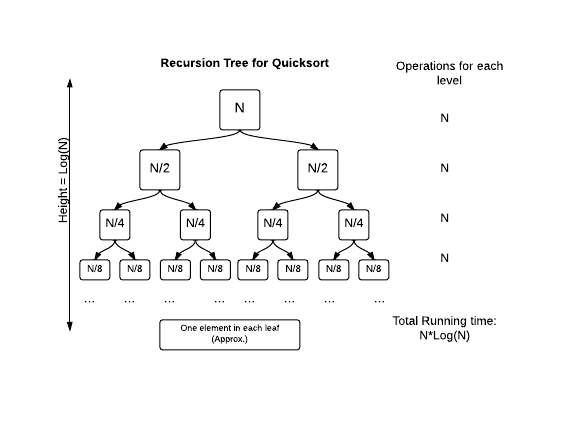
\includegraphics[width=0.68\linewidth]{../images/5450169ba45ae0bd93cbcfde2b1f647259b4606c853e058070134d14cb74b5a9 .png}
\end{figure}
\noindent Quindi si ha che:
\begin{itemize}
    \item \textbf{Radice}: Nel primo nodo più alto c'è il problema inziale: ordinare un array di $n$ elementi
    \item \textbf{Partizione}: l'algoritmo sceglie un pivot e divde l'array in due sotto-array di $ \displaystyle \frac{n}{2}$ elementi:
    \begin{itemize}
        \item elementi minori del pivot
        \item elementi maggiori del pivot
    \end{itemize}
    \item \textbf{Livelli successivi}: ogni sotto-array viene ordinato con un'altra chiamata a Quicksort, quindi l'albero continua:
    \begin{itemize}
        \item livello 0 $\rightarrow$ n
        \item livello 1 $\rightarrow$ $\frac{n}{2}$
        \item livello 2 $\rightarrow$ $\frac{n}{4}$
        \item livello 3 $\rightarrow$ $\frac{n}{8}$
    \end{itemize}
    \item  \textbf{Foglie dell'albero}: L'algoritmo si ferma quando i sotto-array hanno 1 elemento
\end{itemize}
Una volta impostato l'albero di ricorsione basterà quindi sommare i costi di ogni livello e successivamente sommare il costo di ogni livello:
\begin{itemize}[label=$\to$]
    \item Livello 0: c'è un unico nodo di costo $\bm{N}$
    \item Livello 1: ci sono due nodi di costo $\displaystyle  \frac{N}{2}$, quindi il costo del livello è $\displaystyle 2\cdot \left(\frac{N}{2} \right) = \bm{N}$
    \item Livello 2: ci sono quattro nodi di costo $\displaystyle  \frac{N}{4}$, quindi il costo del livello è $\displaystyle 4\cdot \left(\frac{N}{4} \right) = \bm{N}$\\
     $\vdots$
     \item Livello $k$:  ci sono $k$ nodi di costo $\displaystyle  \frac{N}{k}$, quindi il costo del livello è $\displaystyle k\cdot \left(\frac{N}{k} \right) = \bm{N}$
\end{itemize}
Sommando i costi di ogni livello si ottiene che il costo dell'algoritmo nel caso migliore è:
$$T(n) = N \cdot k$$
Ma quanto vale $k$?\\
Per capire quanto vale k (ovvero quanto è alto l'albero della ricorsione) ci dobbiamo chiedere quante volte il valore $N$ può essere diviso per due fino a raggiungere 1. Ciò equivale a dire a quale esponente si deve elevare 2 per ottenere $N$, e questa è proprio la definizione di logaritmo in base 2 di $N$.\\
Quindi il costo totale dell'algoritmo nel caso migliore è:
$$\boxed{T(n) = N\cdot \log_{2}N}$$

\vspace{0.5cm}

\noindent Ora vediamo il \textbf{caso peggiore}: ciò succede quando o la lista è gia ordinata, oppure quando viene scelto un pivot che sia il primo o l'ultimo elemento dell'array. Infatti l'albero di ricorsione sarà degenere (ogni nodo ha al massimo un figlio), poichè l'array viene suddiviso in un sotto-array di dimensione $n-1$, e un sotto-array di 1 elemento. L'albero di ricorsione perciò sarà così:
\begin{figure}[H]
    \centering
    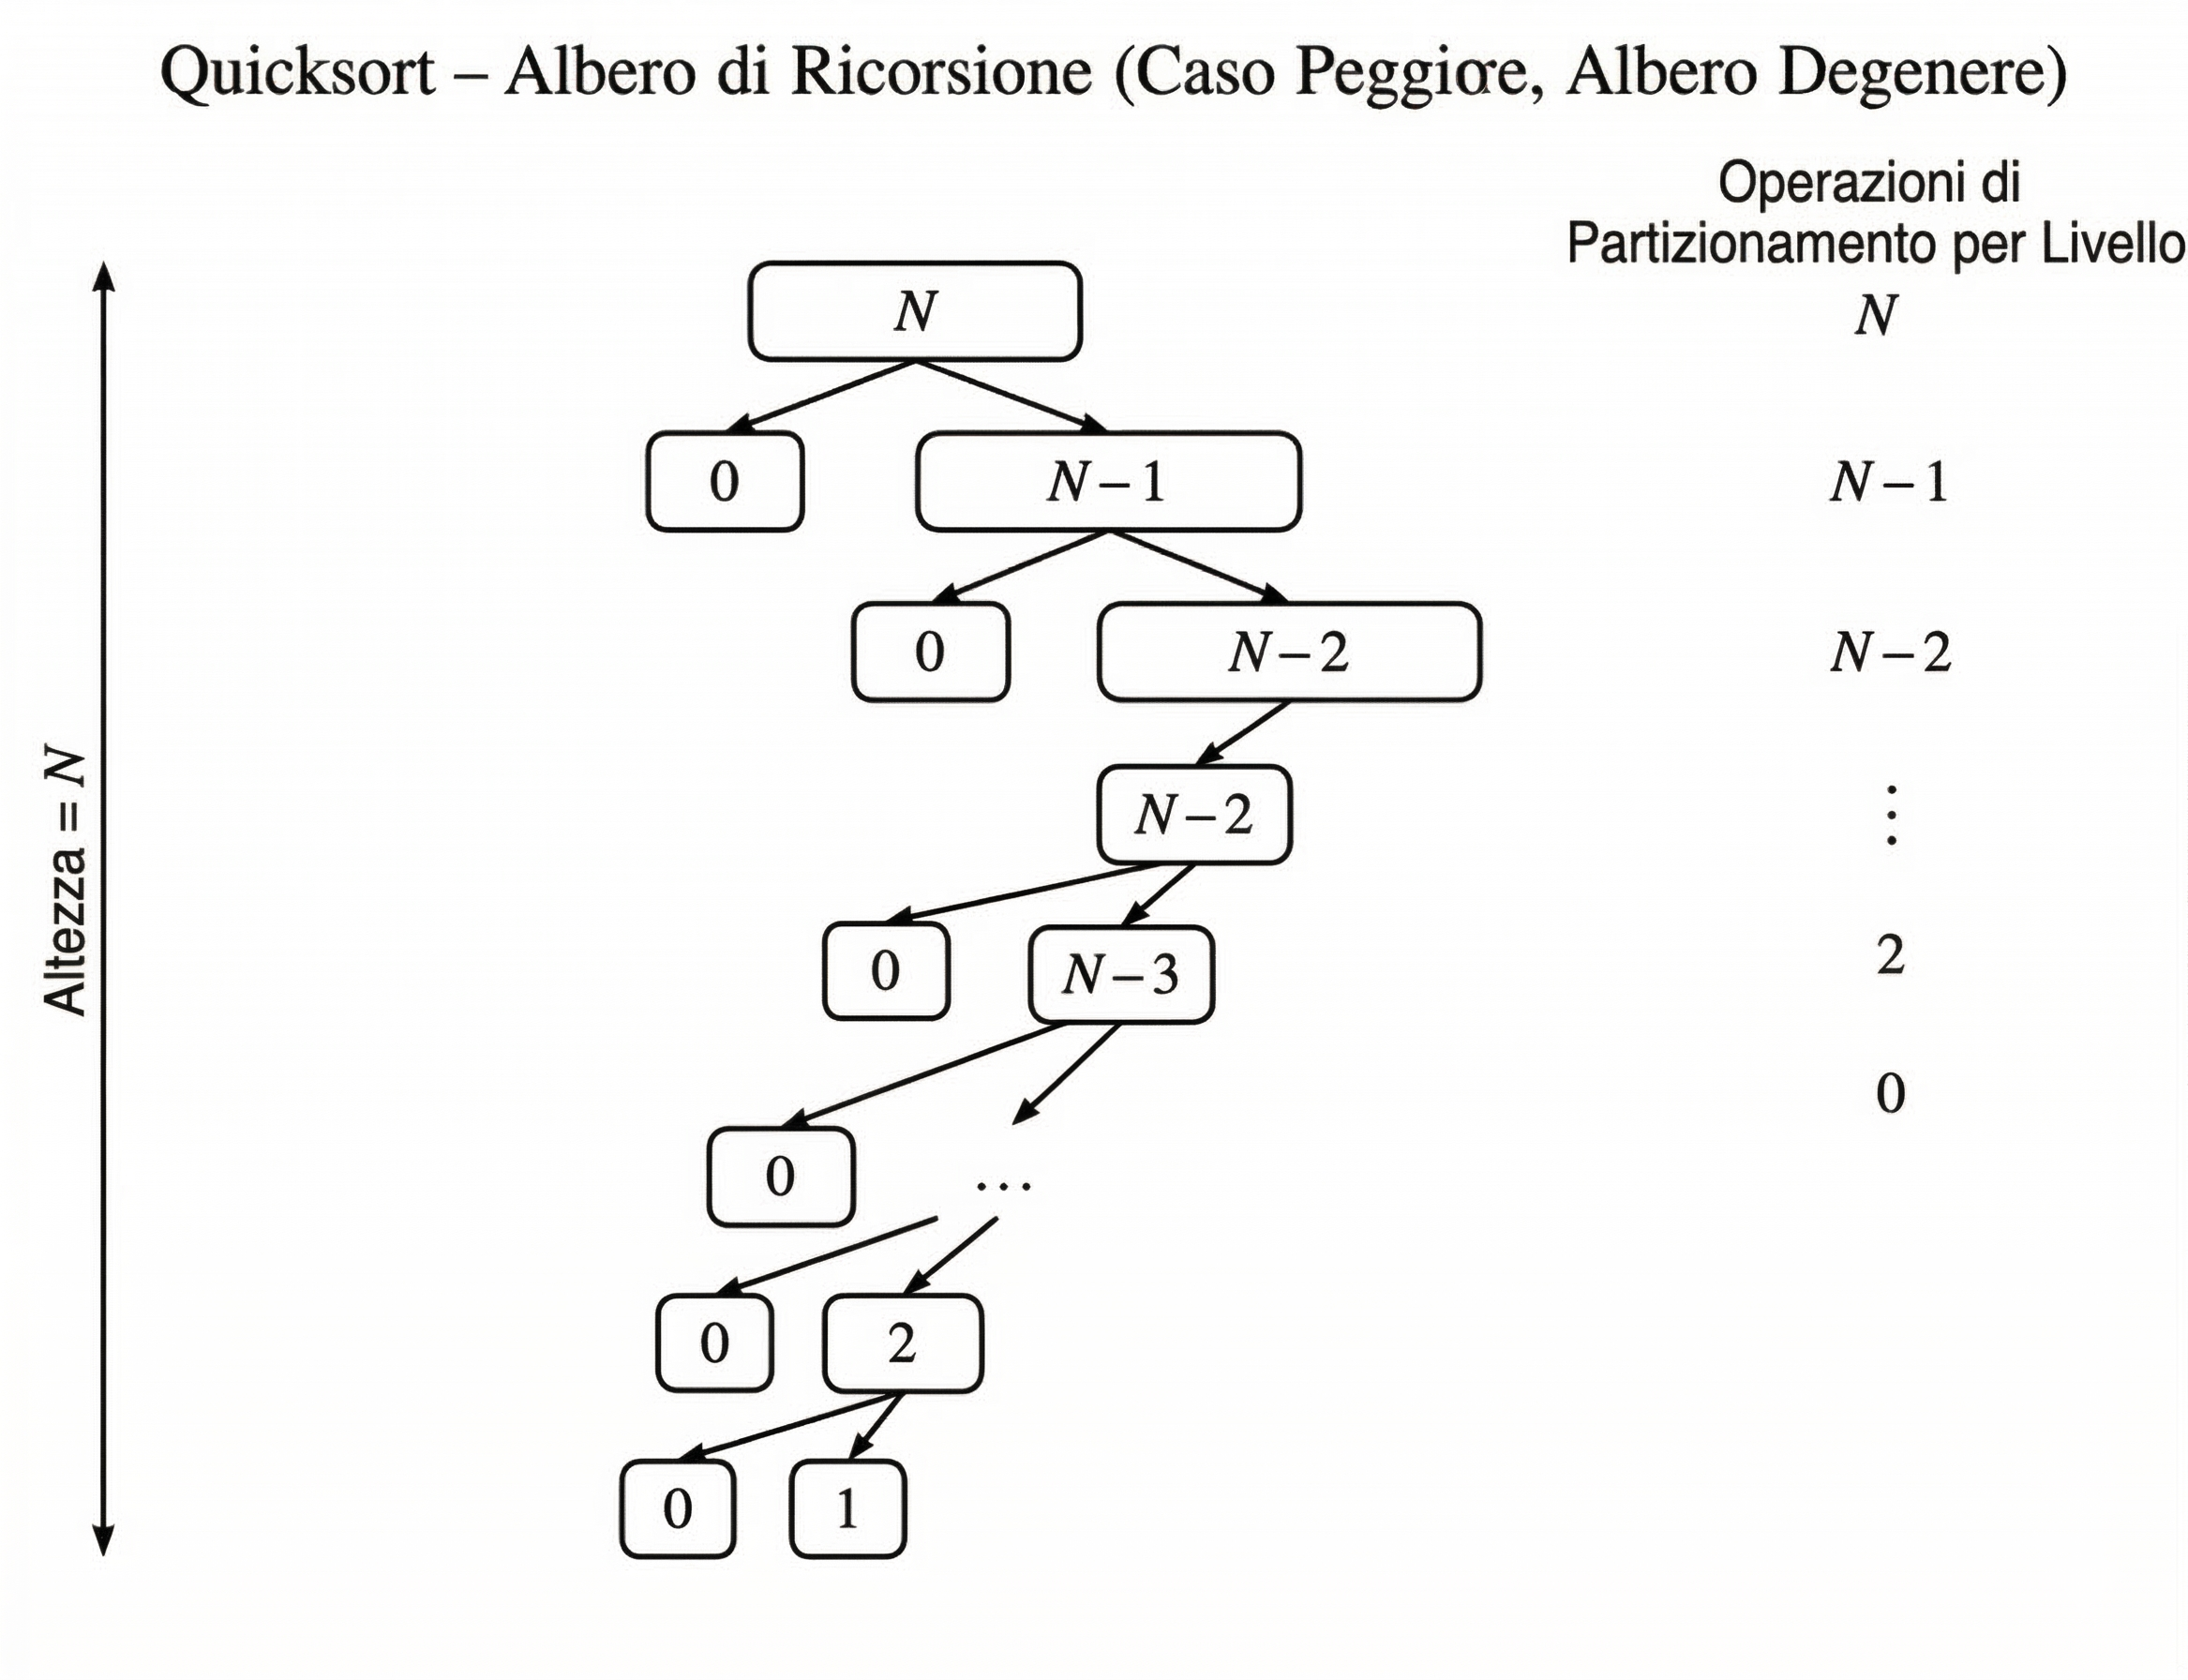
\includegraphics[width=0.5\linewidth]{../images/albero di ricorsione caso peggiore .png}
\end{figure}
In questo caso il costo totale è evidente, in quanto l'albero di ricorsione è alto $N$ e ad ogni livello il costo viene diminuito di 1:
$$T(n) = N\cdot \sum_{i =0}^{k}(N-i)\to \boxed{T(n) \in O(n^2)}$$

\vspace{0.5cm}

\noindent Il \textbf{caso medio} invece, tiene conto della probabilità con cui viene scelto il pivot. Infatti c'è sempre la probabilità del $50\%$ di scegliere un pivot "buono" e il restante $50\%$ di scegliere un pivot "cattivo". Nel caso medio non ci troviamo nè nel caso migliore nè nel caso migliore, quindi l'altezza dell'albero di ricorsione sarà sempre $N\cdot \log N$, ciò che cambia rispetto al caso migliore è che la base del logaritmo non è più $2$, ma dipenderà dalla scelta dei pivot. In generale, comunque, possiamo affermare che il costo nel caso medio è:
$$\boxed{T(n) = N\cdot \log N}$$


\section{Alberi di decisione}
\colorbox{SALZO}{\parbox{\dimexpr\linewidth-2\fboxsep}{\begin{definition}
    (Albero di decisione) Un albero di decisione è un albero pieno (cioè ogni nodo è una foglia oppure ha entrambi i figli), che rappresenta i confronti fra elementi che vengono effettuati da un algoritmo che agisce su un input di una data dimensione. 
\end{definition}}}\smallskip\\
\textit{Osservazione.} Gli alberi di decisione non sono strutture dati.\smallskip\\
L'esecuzione dell'algoritmo di ordinamento corrisponde a tracciare un cammino semplice a partire dalla radice dell'albero di decisione fino ad arrivare ad una foglia. Ogni nodo rappresenta un confronto $a_i \le a_j$. Il sotto-albero sinistro rappresenta i successivi confronti da fare se la condizione $a_i \le a_j$ risulta vera, mentre il sotto-albero destro è dedicato al caso in cui $a_i \le a_j$ non è verificata. Raggiunta una foglia l'algoritmo ha definito un certo ordinamento $a_1\le a_2\le \dots\le a_n$.\\
Siccome qualsiasi algoritmo di ordinamento corretto deve essere in grado di produrre ogni permutazione del suo input, allora una \textbf{condizione necessaria} affinché un ordinamento per confronti sia corretto è che ciascuna delle $n!$ permutazioni di $n$ elementi appaia almeno una volta in una delle foglie dell'albero di decisione. Inoltre ciascuna di queste foglie deve essere raggiungibile dalla radice, attraverso un percorso che corrisponde a una effettiva esecuzione dell'ordinamento per confronti.

\vspace{0.6cm}

\noindent \textit{Esempio.}\\
Vogliamo ordinare un'array di 3 elementi tramite l'algoritmo di Insertion Sort.\\
L'albero di decisione per questo algoritmo è il seguente:
\begin{figure}[H]
    \centering
    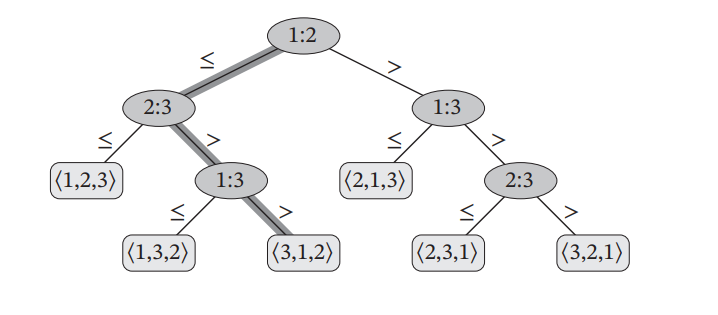
\includegraphics[width=0.5\linewidth]{../images/Albero di decisione .png}
\end{figure}
\textit{Osservazione.} I numeri che sono nei nodi non sono i numeri di con cui sta avvenendo il confronto, ma sono gli indici dell'array di 3 elementi.\smallskip\\
Una volta impostato l'albero di decisione verifichiamo la condizione necessaria, quindi controlliamo che nelle foglie ci siano tutte le possibili permutazioni dell'input: la dimensione dell'array è $n= 3$, quindi ci aspettiamo che nelle foglie ci siano tutte le $n! = 3! = 6$ combinazioni dell'array. Si nota che le 6 permutazioni sono presenti nelle foglie e che sono tutte raggiungibili a partire dalla radice, quindi la condizione necessaria è soddisfatta. Ovviamente il percorso dalla radice alla foglia più corto rappresenta il caso migliore dell'algortimo, analogamente il percorso più lungo (che corrisponde all'altezza dell'albero) rappresenta il caso peggiore.

\subsection{Teorema su alberi di decisione}
\colorbox{SALZO}{\parbox{\dimexpr\linewidth-2\fboxsep}{\begin{theorem}
   Dato un albero di decisione, sia
   \begin{itemize}
       \item $N$: il numero di nodi 
       \item $F$: il numero di foglie
   \end{itemize}
   allora
   $$N = 2F-1$$
\end{theorem}}}\smallskip\\
\textit{Esempio.}\\
Prendiamo in considerazione l'esempio di prima, l'albero di decisione ha 6 foglie, quindi applicando la formula del teorema il numero di nodi è:
$$N = 2F-1 = 2\cdot 6 -1 = \boxed{11}$$

\subsection{Teorema su algoritmi di ordinamento}
\colorbox{SALZO}{\parbox{\dimexpr\linewidth-2\fboxsep}{\begin{theorem}
    Ogni algoritmo di ordinamento per confronti richiede $\Omega (n\log n)$ confronti nel caso peggiore.
\end{theorem}}}
\begin{proof}
    Per stabilire il numero di confronti nel caso peggiore, è sufficiente sapere quanto è alto l'albero di decisione. Consideriamo un albero di decisione di un algoritmo che ha in input $n$ elementi e poniamo:
    \begin{itemize}[label=--]
        \item $H$: valore dell'altezza dell'albero
        \item $L$: numero di foglie 
    \end{itemize}
    Poichè ciascuna delle $n!$ permutazione deve comparire almeno in una foglia (condizione necessaria), si ha che 
    $$n!\le L$$
    Inoltre sappiamo che un albero binario di altezza $H$ non ha più di $2^H$ foglie, si ha che 
    $$n!\le L \le 2^H$$
    Considero la disuguaglianza $n!\le 2^H$ e facendo il logaritmo in base 2 da tutte e due le parti si ottiene:
    $$H \ge \lg (n!) \xrightarrow[]{\text{Approssimazione di Stirling}} \boxed{H = \Omega(n \log n)}$$
\end{proof}


\textbf{Sorting non basato sul confronto}
\section{Counting Sort}
L'algoritmo Counting Sort suppone che ciascuno degli $n$ elementi di input sia un numero intero compreso tra 0 e $k$, per qualche intero $k$. Il Counting Sort per prima cosa determina, per ogni elemento di input $x$, il numero di elementi minori o uguali a $x$, e usa questa informazione per inserire l'elemento $x$ direttamente nella sua posizione nell'array di output. Ecco lo pseudo-codice del Counting-Sort:
\begin{verbatim}
COUNTING-SORT(A, n, k)

1  siano B[1 : n] e C[0 : k] due nuovi array
2  for i = 0 to k
3      C[i] = 0
4  for j = 1 to n
5      C[A[j]] = C[A[j]] + 1
6  // Ora in C[i] c’è il numero di elementi uguali a i.
7  for i = 1 to k
8      C[i] = C[i] + C[i - 1]
9  // Ora in C[i] c’è il numero di elementi minori o uguali a i.
10 // Copia A in B partendo dal fondo di A.
11 for j = n downto 1
12     B[C[A[j]]] = A[j]
13     C[A[j]] = C[A[j]] - 1    // Per gestire valori duplicati
14 return B
\end{verbatim}
L'algoritmo prende in input un'array $A[1:n]$, la dimensione $n$ dell'array e una soglia superiore $k$ sui valori in $A$ (in altre parole $k$ è il valore massimo negli elementi dell'array), che sono interi non negativi. Restituisce l'array $B[1:n]$ che contiene l'output ordinato e usa un array $C[0:k]$ come memoria temporanea di lavoro.\bigskip\\
\textit{Esempio.}\\
Applichiamo l'algoritmo sull'array \texttt{A = [2  5  3  0  2  3  0  3]}, il numero massimo è 5 quindi $k = 5$:
\begin{figure}[H]
    \centering
    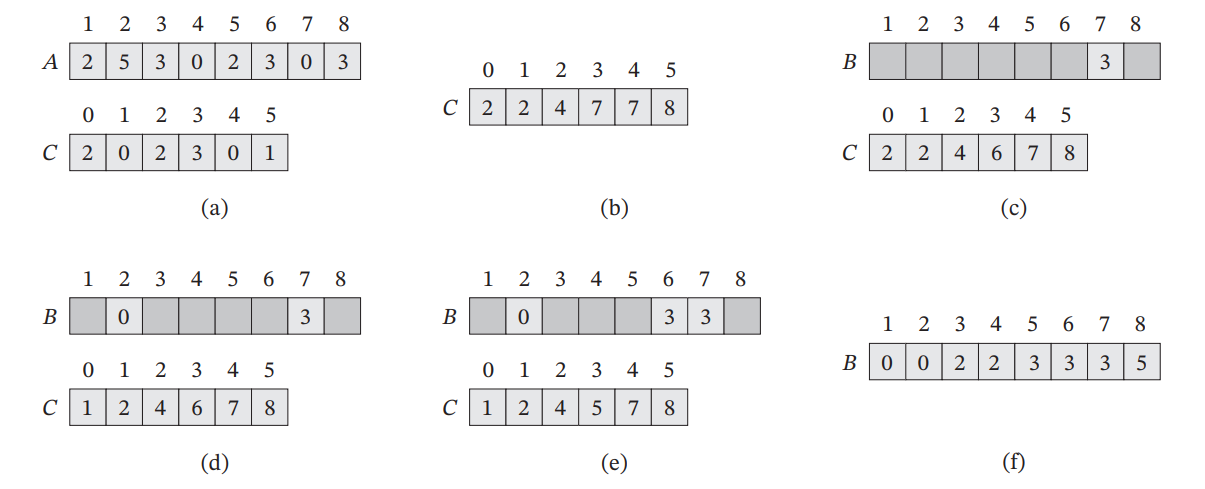
\includegraphics[width=0.9\linewidth]{../images/Counting Sort .png}
\end{figure}
Il funzionamento della procedura Counting Sort su un array di input $A[1 : 8]$, dove ogni elemento di $A$ è un intero non negativo non maggiore di $k = 5$.
\begin{itemize}
    \item[\textbf{(a)}] l’array $A$ e l’array ausiliario $C$ dopo la riga 5.
    \item[\textbf{(b)}] l’array $C$ dopo la riga 8
    \item[\textbf{(c)-(e)}] l’array di output $B$ e l’array ausiliario $C$ dopo, rispettivamente, una, due e tre iterazioni del ciclo (righe 11-13) le caselle di colore grigio chiaro nell’array $B$ rappresentano gli elementi che sono stati inseriti.
    \item[\textbf{(f)}] l’array di output $B$ è ordinato.
\end{itemize}


\section{Bucket sort}
Come il Counting Sort, il Bucket Sort è veloce perchè fa delle assunzioni sull'input. Mentre il Counting Sort suppone che l'input sia formato da interi appartenenti a un intervallo, il bucket sort suppone che l'input sia generato da un processo casuale che distribuisce gli elementi uniformemente e indipendentemente nell'intervallo $[0,1)$.\\
Ciò vuol dire che l'input di array $A[1:n]$ deve rispettare la condizione che ogni elemento $A[i]$ dell'array deve essere tale che:
$$0\le A[i] <1$$
Il Bucket Sort divide l'intervallo [0,1) in $n$ sottointervalli della stessa dimensione, detti \textbf{bucket} (cesti), e poi distribuisce gli $n$ numeri di input nei bucket. Per produrre l'output, ordiniamo i numeri in ogni bucket (attraverso un altro algoritmo di ordinamento), che scorriamo ordinatamente, elencando gli elementi in ciascuno di essi.\smallskip\\
\subsection{Pseudocodice BucketSort}
\begin{verbatim}
BUCKET-SORT(A, n)
1  sia B[0 : n - 1] un nuovo array
2  for i = 0 to n - 1
3      crea la lista vuota B[i]
4  for i = 1 to n
5      inserisci A[i] nella lista B[n · A[i]]
6  for i = 0 to n - 1
7      ordina la lista B[i] con l'insertion sort
8  concatena ordinatamente le liste B[0], B[1], ... , B[n - 1]
9  return la lista concatenata
\end{verbatim}
La supposizione che $0\le A[i] <1$ però può essere limitante per problemi reali dove sono presenti numeri più grandi. Quindi, quando abbiamo valori che sono maggiori di $1$, possiamo comunque usare il Bucket Sort ma bisogna \textbf{normalizzare} l'elemento dell'array prima di metterlo nei bucket. La normalizzazione avviene così:
$$\text{Valore normalizzato} = \frac{\text{Valore attuale} - \text{Valore minimo}}{\text{Valore massimo}- \text{Valore minimo} }$$
Ad esempio, se stiamo ordinando un array di valori tra 10 e 100 e stiamo analizzando il l'elemento $55$, il valore normalizzato sarà:
$$ \text{Valore normalizzato} = \frac{55-10}{100-10} = 0,5$$
E in base a cosa organizziamo gli elementi dell'input nei bucket?\\
Gli elementi vengono organizzati nei bucket calcolando in quale sottointervallo ricade il loro valore. Il numero totale di bucket da creare si sceglie spesso in base alla dimensione dell'input ($n$), ma la regola fondamentale è che tutti i bucket devono coprire un intervallo di valori della stessa identica ampiezza.\\
Infatti il Bucket Sort è particolarmente efficace quando i dati sono distribuiti in modo uniforme su un intervallo.\smallskip\\
Riassumendo, gli step principali del Bucket Sort sono questi:
\begin{enumerate}
    \item \textbf{Distribuzione}: gli elementi vengono distribuiti in diversi bucket in base al loro valore.
    \item \textbf{Ordinamento locale}: ogni bucket viene ordinato separatamente (con un altro algoritmo di ordinamento).
    \item \textbf{Concatenazione}: i bucket ordinati vengono concatenati per ottenere l'output finale.
\end{enumerate}

\subsection{Analisi Bucket Sort}
Sia $n$ la dimensione dell'input e $k$ il costo per produrre l'output.\\ In base al caso in cui ci troviamo avremo costi temporali e spaziali differenti:
\begin{itemize}
    \item \textbf{Caso peggiore}: avviene quando tutti gli elementi dell'input vengono messi nello stesso bucket.
    \begin{itemize}
        \item Costo temporale: $O(n^2)$
        \item Costo spaziale: $O(n+k)$
    \end{itemize}

    \item \textbf{Caso medio}: avviene quando gli elementi dell'input si distribuiscono in maniera non perfettamente uniforme nei bucket.
    \begin{itemize}
        \item Costo temporale: $O(n)$
        \item Costo spaziale: $O(n+k)$
    \end{itemize}

    \item \textbf{Caso ottimale}: avviene quando gli elementi dell'input vengono distribuiti in maniera perfettamente uniforme nei bucket, ovvero ogni bucket ha lo stesso numero di elementi.
    \begin{itemize}
        \item Costo temporale: $O(n)$
        \item Costo spaziale: $O(n+k)$
    \end{itemize}
\end{itemize}

\noindent \textit{Esempio.}\\
Ecco un esempio facendo riferimento allo pseudocodice di Bucket Sort.\\
Si vuole ordinare l'array \texttt{A = [0.78  0.17  0.39  0.26  0.72  0.94  0.21  0.12  0.23  0.68]}
\begin{figure}[H]
    \centering
    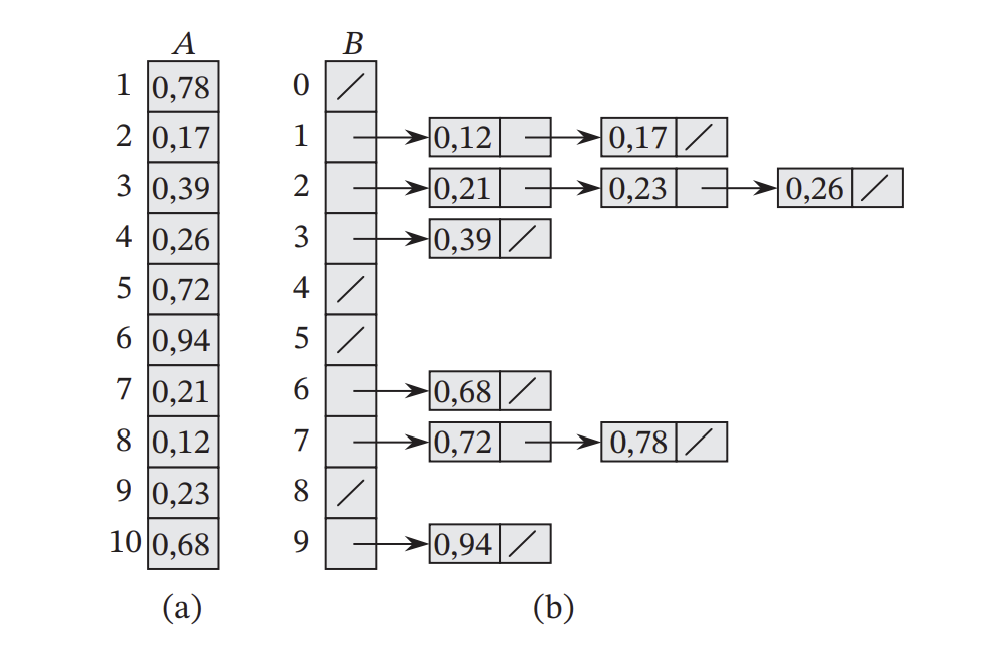
\includegraphics[width=0.58\linewidth]{../images/Esempio Bucket Sort .png}
\end{figure}
\noindent Il funzionamento di Bucket Sort con $n = 10 $ e tutti gli elementi compresi tra 0 e 1, quindi non c'è bisogno della normalizzazione.
\begin{itemize}
    \item [\textbf{(a)}] L'array di input $A[1:10]$
    \item [\textbf{(b)}] L'array $B[0:9]$ formato da liste ordinate (i bucket) dopo l'esecuzione della riga 7 dell'algoritmo, le barre \texttt{"/"} indicano la fine di ciascun bucket. L'i-esimo bucket contiene i valori che cadono nell'intervallo semiaperto $\left[ \frac{i}{10},\frac{(i+1)}{10}  \right]$. L'output ordinato è formato dalla concatenazione è formato dalla concatenazione ordinata delle liste $B[0],\ B[1], \dots , B[9]$.
\end{itemize}


\section{Radix Sort LSD}
Il Radix Sort LSD (Least Significant Decimal) è un algoritmo di ordinamento per valori numerici interi. Questo algoritmo risolve il problema dell'ordinamento dei numeri in maniera controintuitiva, ordinando prima i numeri in base alla cifra meno significativa. Concretamente, vogliamo ordinare dei numeri aventi $d$ cifre, mettiamo in colonna i numeri e prendiamo in considerazione la colonna delle cifre meno significative (quindi la colonna tutta a destra) e ordiniamo i numeri a seconda dell'ordinamento delle cifre in quella colonna.\\ 
Vediamo un esempio numerico:\smallskip\\
\textit{Esempio.}\\
Dobbiamo ordinare i seguenti numeri: \texttt{329  457  657  839  436  720  355}
\begin{figure}[H]
    \centering
    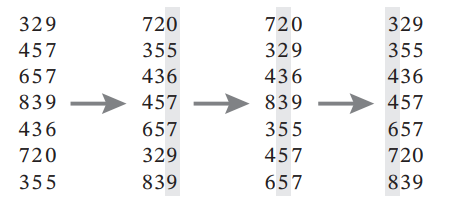
\includegraphics[width=0.5\linewidth]{../images/Esempio Radix Sort.png}
\end{figure}

\vspace{1cm}

\noindent Il codice per il Radix Sort è semplice, l'algoritmo suppone che ogni elemento nell'array $A[1:n]$ abbia $d$ cifre, dove la cifra 1 è quella di ordine pià basso e la cifra $d$ è quella di ordine più alto. Ecco il codice:
\begin{verbatim}
    for i = 1 to d
        usa un ordinamento stabile per ordinare l'array A[1:n]
        rispetto alla cifra i
\end{verbatim}
È essenziale che gli ordinamenti delle cifre in questo algoritmo siano \textbf{stabili}.\\
Ma cosa vuol dire che un algoritmo di ordinamento deve essere stabile?\smallskip\\
\colorbox{SALZO}{\parbox{\dimexpr\linewidth-2\fboxsep}{\begin{definition}
    (Algoritmo stabile) Un algoritmo di ordinamento è stabile se preserva le relazioni delle posizioni fornite come input.
\end{definition}}}\smallskip\\
Per capire meglio facciamo un esempio:\smallskip\\
\textit{Esempio.}\\
Devo ordinare i seguenti numeri: \texttt{3  1*  2  1}\\
Nell'array ci sono due 1, quindi se l'algoritmo è stabile allora viene preservato l'ordine degli 1 e l'output sarà:
\begin{center}
    \texttt{1*  1  2  3}
\end{center}
Altrimenti l'algoritmo è considerato non stabile.

\section{Riduzione (fra problemi)}
\colorbox{SALZO}{\parbox{\dimexpr\linewidth-2\fboxsep}{\begin{definition}
    (Riduzione fra problemi) Nel campo degli algoritmi, ridurre un Problema $A$ a un Problema $B$ significa trasformare un'istanza del Problema $A$ in un'istanza del Problema $B$, in modo da poter usare un algoritmo che risolve $B$ per risolvere anche $A$.
\end{definition}}}

\section{HeapSort}
\subsection{Definizione Heap}
Un Heap è una struttura dati, basata su alberi binari, ovvero alberi che possono avere al massimo due figli. Queste strutture possono essere rappresentate mediante array i cui elementi sono i nodi dell'albero.\\
\textbf{proprietà}
\begin{itemize}
    \item ogni elemento dell'albero corrisponde ad un elemento dell'array
    \item tutti i livelli dell'albero sono completamente riempiti salvo l'ultimo che può essere parzialmente riempito da sinistra fino ad un certo punto.
\end{itemize}

\begin{figure}[H]
    \centering
    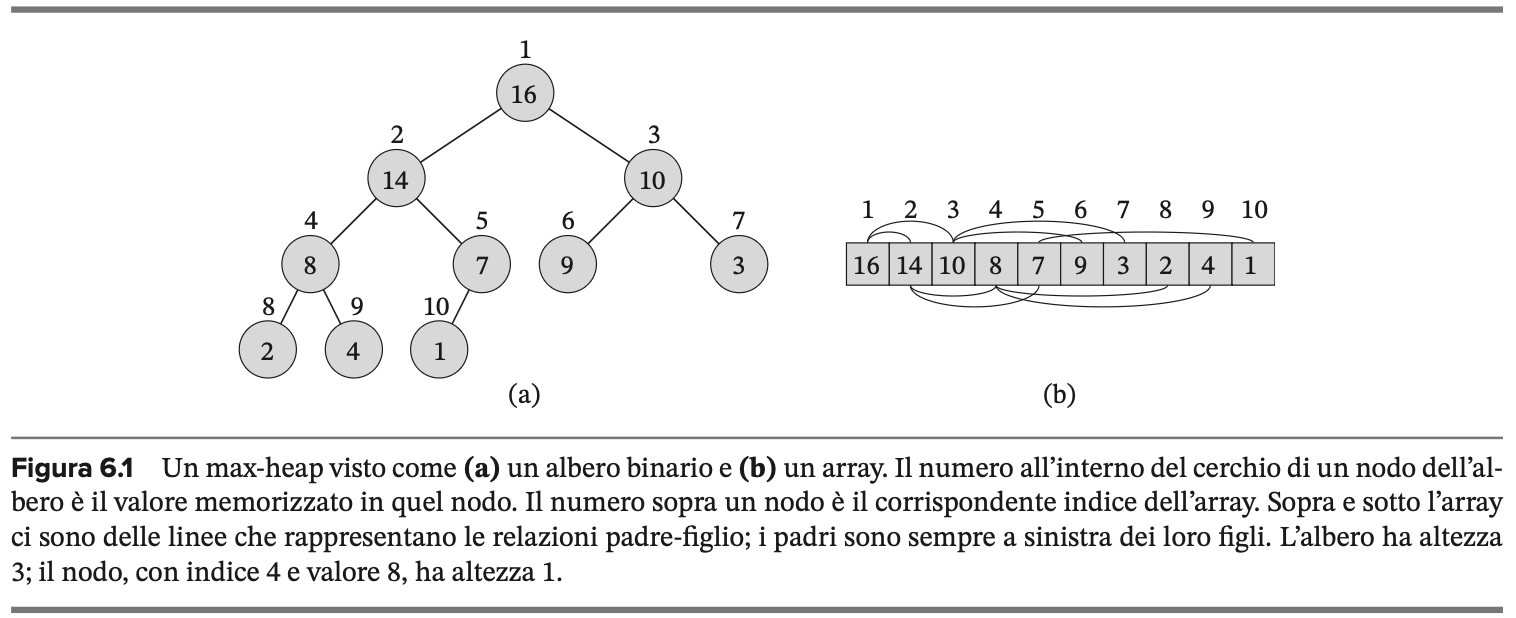
\includegraphics[width=0.75\linewidth]{../images/max-heap.png}
\end{figure}
\noindent Un heap è rappresentato da un oggetto che contiene
\begin{itemize}
    \item un array di elementiA[1,n]
    \item un intero size (tale che $0 \le size \le n$)
\end{itemize}
\noindent Un array A che rappresenta un heap ha due attributi specifici: \textbf{A.lenght} che indica il numero di elementi dell'array e \textbf{A.heapSize} che indica il numero di elementi dell'array che appartengono all'heap. In generale si ha che $0 \le A.heapSize \le A.lenght$.\\
Per ogni elemento i dell'array, ad eccezione della radice che è l'elemento $A[1]$, è possibile determinare il padre e i suoi due figli, in particolare:\\
PARENT(i) = $\lfloor \frac{1}{2} \rfloor$\\
LEFT(i) = 2i\\
RIGHT(i) = 2i+1

\subsection{Max-heap e Min-heap}
Esistono due tipi particolari di heap chiamati mex-heap e min-heap.\\
Un \textbf{max-heap} è un heap in cui, per ogni nodo i diverso dalla radice, abbiamo che $A[PARENT(i)] \ge A[i]$, ovvero il padre è maggiore del figlio.\\
Un \textbf{min-heap} è un heap in cui, per ogni nodo i diverso dalla radice, abbiamo che $A[PARENT(i)] \le A[i]$, ovvero i figli sono maggiori del padre.\\
\textbf{Osservazione}\\
In un max-heap la radice rappresenta il massimo.\\
In un min-heap la radice rappresenta il minimo.\\
\textbf{Esempio:}\\
Dato l'array\\
\begin{figure}[H]
    \centering
    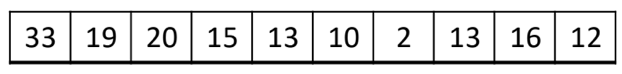
\includegraphics[width=0.5\linewidth]{../images/esempio-max-heap.png}
\end{figure}
\noindent determinare il max-heap:\\
\begin{figure}[H]
    \centering
    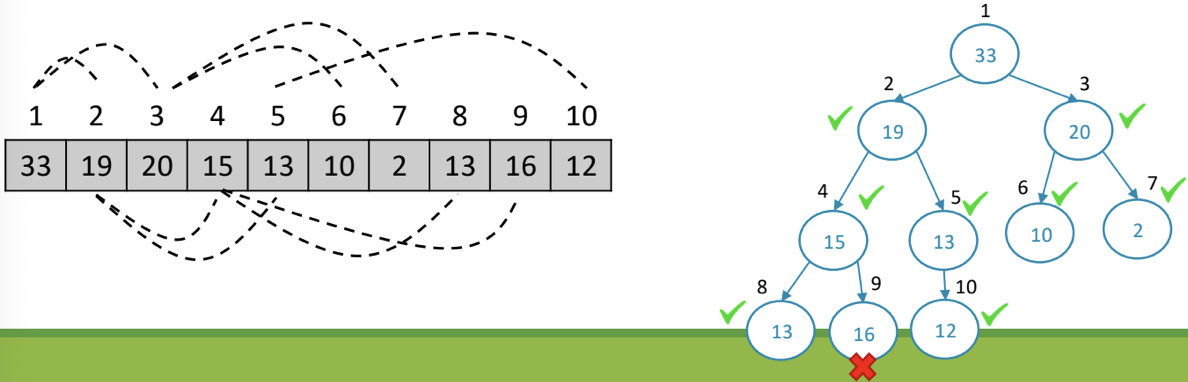
\includegraphics[width=0.5\linewidth]{../images/esempio-max-heap2.png}
\end{figure}

\subsection{Max-Heapify}
L'heap memorizza elementi e può essere modificato.
Per non perdere proprietà durante le modifiche  della strutture dati utilizziamo l'algoritmo MAX-HEAPIFY(A,i) che si occupa di costruire un max-heap con radice nel nodo i.
\subsubsection{pseudocodice MAX-HEAPIFY(A,i)}
\begin{verbatim}
MAX-HEAPIFY(A,i)
1   l = left(i)
2   r = right(i)
3   if i <= A.heapSize AND A[l]  > A[i]
4       largest = i
5   else largest = i
6   if r <= A.shapeSize AND A[r] > A[largest]
7       largest = r
8   if largest != i
9       scambia A[i] con A[largest]
10  MAX-HEAPIFY(A,largest)
\end{verbatim}
\noindent \textbf{Funzionamento}\\
Quando viene chiamata questa funzione, si assume che i sottoalberi con radici \textbf{left(i)} e \textbf{right(i)} siano max-heap, mentre non è certo che il padre \textbf{i} sia effettivamente più grande dei figli. Vengono salvati gli indici del figlio sinistro e del figlio destro, dopodiché si procede a verificare innanzitutto se questi indici sono nei limiti dell'array e se viene rispettata la condizione $A[i]>A[l]$ e $A[r]$, se così non fosse verrebbe salvato nella variabile \textbf{largest} l'indice del figlio maggiore e verrebbero scambiati A[largest] e il padre.\\
Così facendo la condizione di un max-heap sarebbe verificata per la terna appena considerata, tuttavia potrebbe non essere verificata nel sottoalbero che ha come radice il nodo appena scambiato, allora si procede a richiamare ricorsivamente la funzione sull'indice di largest, ovvero il nodo appena scambiato. Dunque, in breve, si fa scendere il valore $A[i]$ nel max-heap in modo che il sottoalbero con radice di indice $i$ diventi un max-heap.\\
\begin{figure}[H]
    \centering
    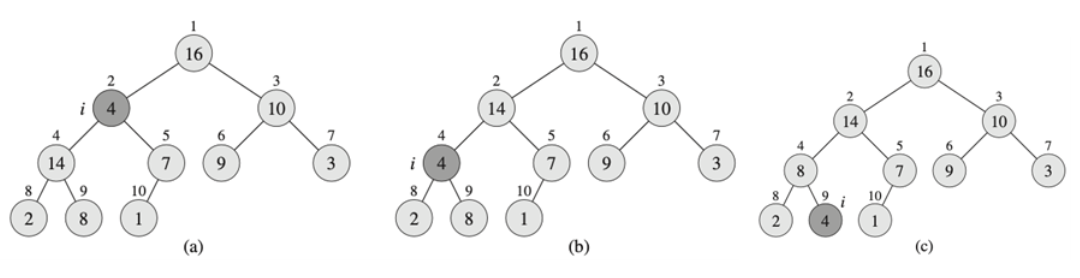
\includegraphics[width=0.75\linewidth]{../images/max-heapify.png}
    
\end{figure}
\begin{figure}[H]
    \centering
    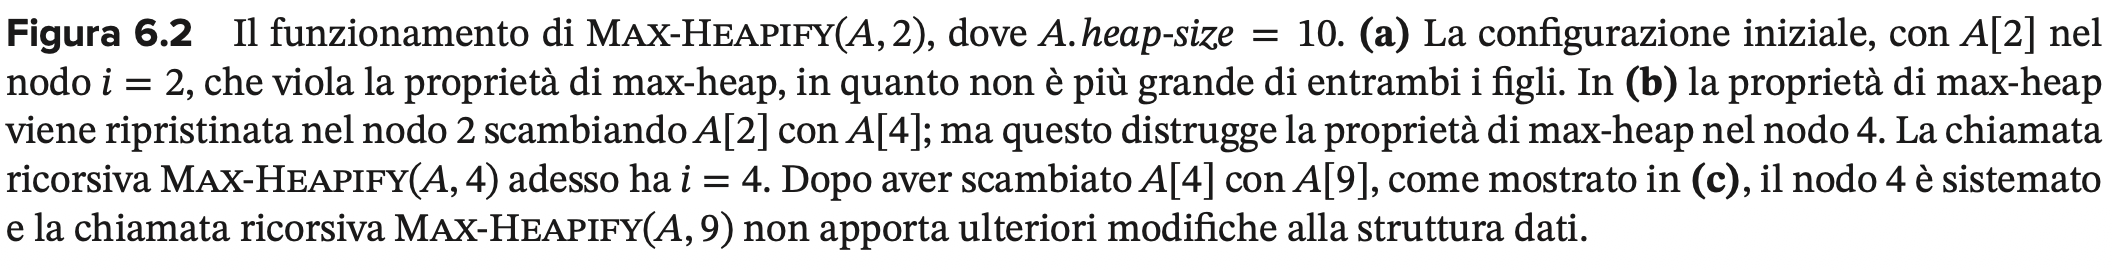
\includegraphics[width=0.75\linewidth]{../images/funzionamento-max-heapify.png}
    
\end{figure}
\noindent \subsubsection{costo}
dalla riga a 9 faccio solo confronti perciò ha costo O(1), mentre la chiamata ricorsiva fatta al più h volte, dove h è l'altezza del sottoalbero $(< \log n)$. Quindi ha costo \textbf{O(h)}.\\
\subsection{Costruire un max-heap}
La procedura Build-Max-Heap eseguita in un tempo lineare, genera da un array di input non ordinato un max-heap;
\begin{verbatim}
BUILD-MAX-HEAP(A,n)
1   A.heapSize = n
2   for i = [n/2] down to 1
3       MAX-HEAPIFY(A,i)
\end{verbatim}
\noindent \textbf{Funzionamento}\\
La funzione Max-Heapify può essere utilizzata in modo alternativo, ovvero dal basso verso l'alto, per convertire un array di input con n = A.length in un max-heap. E' possibile utilizzare la funzione Max-Heapify poiché gli ultimi elementi di ciascun sottoalbero possono essere considerati foglie dell'albero, dunque si parte da esse per salire verso la radice. Build-Max-Heap si limita a richiamare iterativamente Max-Heapify su A passando l'indice i che varia dalla metà dell'array decrementato fino ad 1, così facendo fa salire nell'albero i valori più grandi e fa scendere quelli più bassi.
\begin{figure}[H]
    \centering
    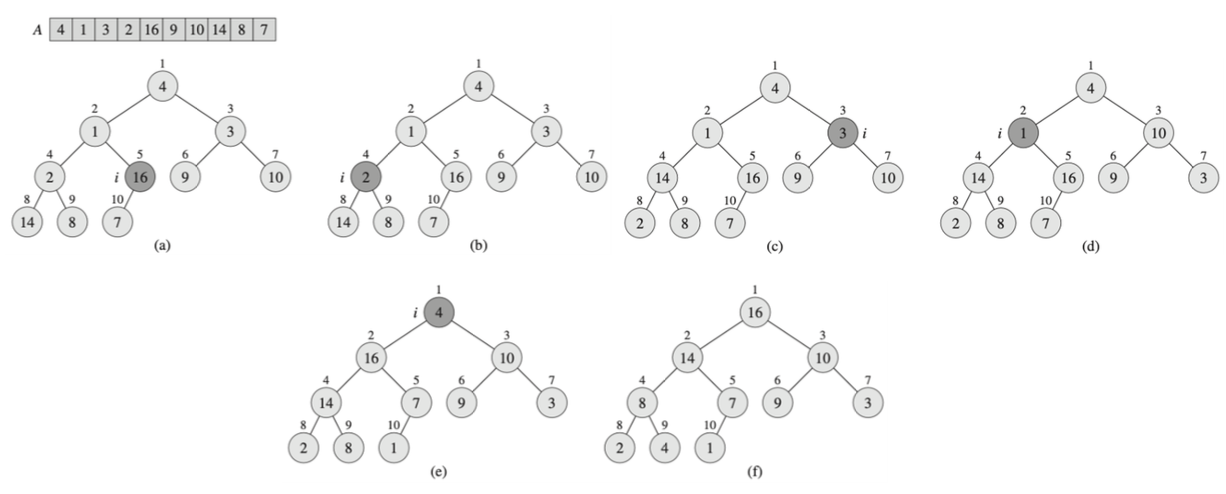
\includegraphics[width=0.75\linewidth]{../images/buil-max-heap.png}
\begin{figure}[H]
        \centering
        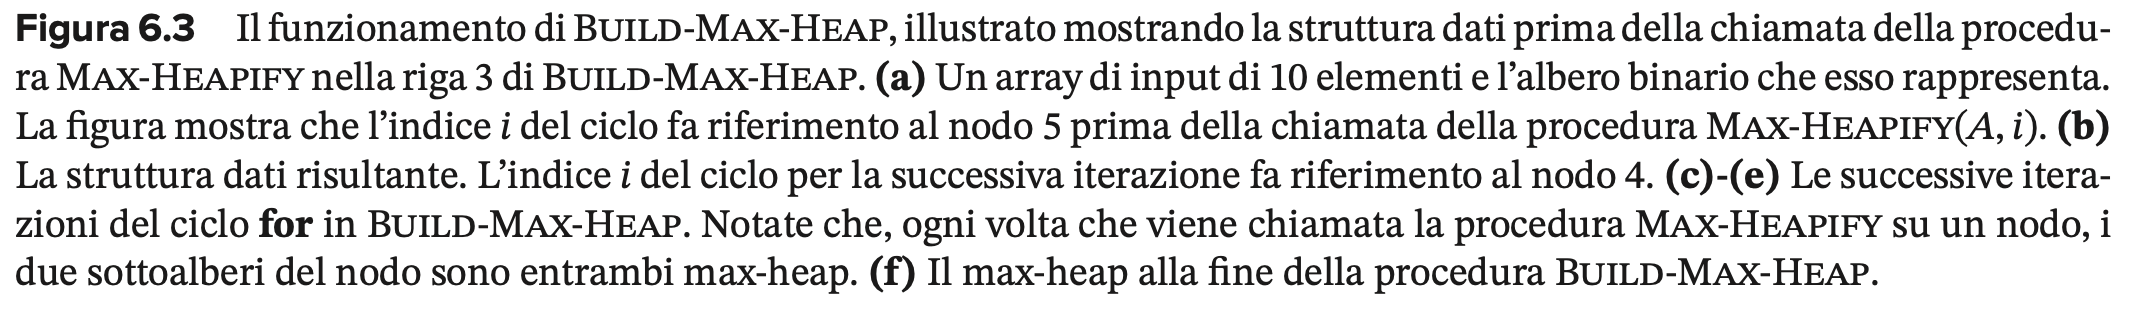
\includegraphics[width=0.75\linewidth]{../images/funzionamento-buil-max-heap.png}
       
    \end{figure}
        
\end{figure}

\noindent \subsubsection{costo}
Upper bound $O(n \log n)$ perché MAX-HEAPIFY mi costa $\log n$ e lo ripeto al più n volte\\
Questo limite superiore sebbene corretto, non è asintoticamente stretto.\\
Possiamo ottenere un limite più stretto osservando che il tempo per eseguire Max-Heapify in un nodo varia con l'altezza del nodo nell'albero, e le altezza della maggior parte di essi sono più piccole. L'analisi più rigorosa si basa sulle proprietà che un heap di n elementi ha altezza $\lfloor \log n \rfloor$ e, per ogni h,ha al più $\lceil n/2^{h+1} \rceil$ nodi di altezza h.
Il tempo richiesto dalla procedura Max-Heapify quando viene chiamata per un nodo di altezza $h$ è $O(h)$. Possiamo dire che il costo totale di build-Max-Heap è limitato superiormente da\\
$\sum_{h=0}^{ \lfloor \log n \rfloor} \lceil \frac{n}{2^{h+1}} \rceil O(h)=O(n \sum_{h=0}^{ \lfloor \log n \rfloor} \frac{h}{2^h})$\\
con $\sum_{h=0}^{ \lfloor \log n \rfloor} \frac{h}{2^h} \rightarrow \sum_{h=0}^\infty \frac{h}{2^h}=\frac{1/2}{(1-1/2)^2}=2$\\
Perciò ho $O(n)$.
\subsubsection{Correttezza di Build-Max-Heap}
Per verificare che Build-Max-Heap funziona correttamente, utilizziamo la seguente invariante di ciclo.\\
\texttt{All'inizio di ogni iterazione del ciclo for, righe 2-3, ognuno dei nodi i+1, i+2,...,n è la radie di un max-heap}\\
\textbf{Inizializzazione}\\
Prima della prima iterazione del cicl, $i =\lfloor n/2 \rfloor$\\. Ognuno dei nodi $\lfloor n/2 \rfloor + 1$, $\lfloor n/2 \rfloor + 2$,...,$n$ è una foglia e, quindi, è la radice di un max-heap con un solo nodo. \\
\textbf{Mantenimento}\\
per verificare che ogni iterazione conserva l'invariante di ciclo, notiamo che i figli del nodo $i$ hanno una numerazione più alta di $i$. Per l'invariante di ciclo, quindi, essi sono entrambi radici di un max-heap. Questa è esattamente la condizione richiesta affinché la chiamata Max-Heapify(A,i) renda il nodo $i$ la radice di un max-heap. Inoltre, la chiamata di Max-Heapify preserva la proprietà che tutti i nodi $i+1,i+2,..,n$ siano radici di un max-heap. Il fatto che $i$ venga decrementato di un'unità a ogni iterazione del ciclo for ristabilisce l'invariante di ciclo per la successiva ietrazione. \\
\textbf{Conclusione}\\
Il ciclo esegue esattamente $\lfloor n/2 \rfloor$ iterazioni, e quindi termina. Alla fine del ciclo si ha $i=0$. Per l'invariante di ciclo, ognuno dei nodi 1,2,...,n è la radice di un max-heap; in particolare, lo è il nodo 1.
\subsection{Heap Sort}
Che eseguita in un tempo $O(n \log n)$, ordina un array.
\begin{verbatim}
HeapSort(A,n)
1   BUILD-MAX-HEAP(A,n)
2   for i = n down to 2
3       scambia A[1] con A[i]
4       A.heapSize = A.heapSize-1
5       MAX-HEAPIFY(A,1)
\end{verbatim}
\noindent \textbf{Funzionamento}\\
La funzione HeapSort chiama inizialmente Build-Max-Heap(A, n) per trasformare A in un max-heap. Dunque, se per definizione l’elemento più grande dell’array è memorizzato nella radice A[1], per ordinare in modo crescente l’albero, basta scambiare la radice con l’elemento in posizione finale, ovvero A[n]. Dopodichè si decrementa A.heapSize, in modo tale da non considerare più l’elemento in ultima posizione, in quanto si trova nella sua posizione definitiva. Per ottenere un max-heap basta chiamare Max-Heapify(A, 1) per far tornare il max alla radice. Questo ciclo viene ripetuto n-1 volte. Build-Max-Heap impiega \textbf{O(n)}, mentre
Max-Heapify \textbf{O(log n)}, in totale il costo di HeapSort ammonta a \textbf{O(n log n)}.